%%%%%%%%%%%%%%%%%%%%%%%%%%%%%%%%%%%%%%%%%%%%%%%%%%%%%%%%%%%%%%%%%%%%%%%%%%%%%%%%%%%%%%%%%%
%% Document Class: thesis
%% Created by: Jeremy West, April 2009
%% Document Options: see the standard report class for LaTeX, they are all the same
\documentclass[12pt]{thesis}
% \usepackage{amsmath}
\usepackage{overpic}
\usepackage{amsthm,amsmath,amsfonts,amssymb,amscd,mathrsfs}
\usepackage{graphicx}
\usepackage{float}
\usepackage{bbm} %\mathbb numbers and other symbols
\usepackage{caption}
\usepackage{subcaption}
% \usepackage{bm} % \boldsymbol
% \usepackage{hyperref}

%%%%%%%%%%%%%%%%%%%%%%%%%%%%%%%%%%%%%%%%%%%%%%%%%%%%%%%%%%%%%%%%%%%%%%%%%%%%%%%%%%%%%%%%%%
%% Document Properties
%% PLEASE SET THESE TO THE APPROPRIATE VALUES FOR YOUR THESIS
\author{Ethan Walker} %MAKE SURE THAT YOUR NAME MATCHES THE ONE ON YOUR OFFICIAL BYU RECORD.
\title{Network Specialization: A Topological Mechanism for the Emergence of Cluster Synchronization}
%The title must be mixed case letters and located one inch from the top edge of the page. Titles Must Be in Mixed Case and May Not Exceed Six Inches on One Line and Must Be in the Inverted Pyramid Format When Additional Lines Are Needed. Prepositions of more than five letters should be capitalized.
\degree{Master of Science} % e.g. Master of Science, Doctor of Philosophy  MAKE SURE THE THESIS.CLS FILE MATCHES THIS.
\university{Brigham Young University} % e.g. Brigham Young University
\department{Department of Mathematics} % e.g. Department of Mathematics
\committeechair{Benjamin Webb} % that is, your advisor. DO NOT USE TITLES OR DEGREE ABBREVIATIONS AFTER NAMES.
\year{2022}
%% These are fields that are stored in the PDF but are not visible in the document
%% itself. They are optional. The first is the subject of your thesis (like algebraic geometry)
\memberA{Mark Kempton}
\memberB{Todd Fischer}
%\memberC{4th member if you're writing a dissertation}
%\memberD{5th dissertation member}
\subject{Network Science}
%% The keywords should be a comma-separated list: math, cool stuff, my research... Only proper nouns (i.e. names) should be capitalized.
\keywords{networks, network science, synchronization, dynamical systems, dynamical networks}
%%%%%%%%%%%%%%%%%%%%%%%%%%%%%%%%%%%%%%%%%%%%%%%%%%%%%%%%%%%%%%%%%%%%%%%%%%%%%%%%%%%%%%%%%%

\pdfbookmarks
%% This creates an index (if you use the MakeIndex program). Comment it out if you
%% don't want and index.
% \makeindex

%% This file contains the theorem definitions and custom commands that I commonly use
%% they may be changed, the reference to the file removed, etc. Or, if you like, you 
%% may use them as well.

%% Define the theorem styles and numbering
\theoremstyle{plain}
\newtheorem{theorem}{Theorem}[chapter]
\newtheorem{proposition}[theorem]{Proposition}
\newtheorem{conjecture}[theorem]{Conjecture}
\newtheorem{corollary}[theorem]{Corollary}
\newtheorem{lemma}[theorem]{Lemma}

\theoremstyle{definition}
\newtheorem{definition}[theorem]{Definition}
\newtheorem{example}[theorem]{Example}

\theoremstyle{remark}
\newtheorem*{remark}{Remark}

%% Create shortcut commands for various fonts and common symbols
\newcommand{\s}[1]{\mathcal{#1}}
\newcommand{\N}{\mathbb{N}}
\newcommand{\Z}{\mathbb{Z}}
\newcommand{\Q}{\mathbb{Q}}
\newcommand{\R}{\mathbb{R}}
\newcommand{\C}{\mathbb{C}}
\newcommand{\F}{\mathbb{F}}

%% Declare custom math operators
\DeclareMathOperator{\tr}{tr}
\DeclareMathOperator{\diag}{diag}
\DeclareMathOperator*{\argmin}{argmin}
\DeclareMathOperator*{\argmax}{argmax}
\DeclareMathOperator{\Span}{Span}
\DeclareMathOperator{\rank}{rank}

%% Sets and systems
\newcommand{\br}[1]{\left\langle #1 \right\rangle}
\newcommand{\paren}[1]{\left(#1\right)}
\newcommand{\sq}[1]{\left[#1\right]}
\newcommand{\set}[1]{\left\{\: #1 \:\right\}}
\newcommand{\setp}[2]{\left\{\, #1\: \middle|\: #2 \, \right\}}
\newcommand{\abs}[1]{\left| #1 \right|}
\newcommand{\norm}[1]{\left\| #1 \right\|}
\newcommand{\system}[1]{\left\{ \begin{array}{rl} #1 \end{array} \right.}

%% referencing commands
\newcommand{\thmref}[1]{Theorem \ref{#1}}
\newcommand{\corref}[1]{Corollary \ref{#1}}
\newcommand{\lemref}[1]{Lemma \ref{#1}}
\newcommand{\propref}[1]{Proposition \ref{#1}}
\newcommand{\defref}[1]{Definition \ref{#1}}
\newcommand{\exampleref}[1]{Example \ref{#1}}
\newcommand{\exerref}[1]{Exercise \ref{#1}}

% set the labeling style
\renewcommand{\labelenumi}{(\roman{enumi})}


\begin{document}

\setlength{\abovedisplayskip}{3pt}
\setlength{\belowdisplayskip}{3pt}

%%%%%%%%%%%%%%%%%%%%%%%%%%%%%%%%%%%%%%%%%%%%%%%%%%%%%%%%%%%%%%%%%%%%%%%%%%%%%%%%%%%%%%%%%%
%% \frontmatter sets the page numbering to roman for the introductory pages
\frontmatter
\maketitle  % make the title page

%% Your abstract goes in here
\begin{abstract} %leave a blank line between abstract and first paragraph. 

%The paragraphs of the abstract should be indented. This is part of the template, but in case it doesn't work, you'll need to but a \qquad at the front of the first paragraph.
\qquad Real-world networks are dynamic in that both the state of the network components and the structure of the network (topology) change over time. 
Most studies regarding network evolution consider either one or the other of these types of network processes.
Here we consider the interplay of the two, specifically, we consider how changes in network structure effect the dynamics of the network components.
To model the growth of a network we use the specialization model known to produce many of the well-known features observed in real-world networks. 
We show that specialization results in a nontrivial equitable partition of the network where the elements of the partition form clusters that have synchronous dynamics.
In particular, we show that these synchronizing clusters inherit their ability to either locally or globally synchronize from the subnetwork from which they are specialized.
Thus, network specialization allows us to model how dynamics and structure can co-evolve in real-world systems.

\vskip 4.5in
 
\noindent Keywords: networks, network science, synchronization, dynamical systems, dynamical networks %Keywords need to be as close to the bottom of the page as possible without moving to a new page.
\end{abstract}


%% Your acknowledgements go here, comment this out if you don't want them
\begin{acknowledgements}
\qquad I'd like to thank the Dr.~Webb for his assistance, without his help this would not have been completed.
Thank you to my committee for their attentive eye and insightful questions.
Thank you to Dr.~Jarvis, your immense patience and support have been life changing.
Thank you to my family and friends that have supported me throughout my education, I am forever indebted to those that have gone before me.
\end{acknowledgements}

%The following is an OPTIONAL signature page and SHOULD NOT be included in the PDF file submitted to the ETD program.
% Use this to describe your committee. You have already specified your committee chair above.
% List each additional member using the \member command as illustrated.
%\begin{committee}
%	\member{Just A. Member}  % The name of the faculty member as you would like it to appear
%	\member{A. Good Prof}
%	\member{A long professors name, perhaps with a \\ line break in it}
%	\member{Maybe one more person}

% 
%     \member{Lennard Bakker, Graduate Coordinator}
%     \member{Gus Hart, Associate Dean\\
%     College of Physical and Mathematical Sciences}
%\end{committee}

%% These create the obvious pieces: table of contents, list of tables, list of figures.
%% Comment them out if you don't want them
\tableofcontents
% \listoftables
\listoffigures

%%%%%%%%%%%%%%%%%%%%%%%%%%%%%%%%%%%%%%%%%%%%%%%%%%%%%%%%%%%%%%%%%%%%%%%%%%%%%%%%%%%%%%%%%%
%% This is where the body of the thesis begins. \mainmatter turns on the standard numbering
%% and headers
\mainmatter

\chapter{Introduction}\label{chapt:intro}
Networks studied in the biological, social and technological sciences are inherently dynamic.
Periodic dynamics related to circadian rhythms and life cycles are a hallmark of biological networks \cite{1}.
Synchronizing patterns of dynamics are found in the heart and brain \cite{2} and synchronization is used in telecommunication networks to measure service quality \cite{3,4}.
Stable and multistable dynamics are observed in cellular differentiation, metabolic, and other networks \cite{5,6}. 

Aside from the changing state of network components, over longer time-scales networks are also dynamic in terms of their topology \cite{7}.
Individuals move in and out of social networks, websites and the hyperlinks between them are updated, and the neural connections in the brain are rewired presumably to allow for improved processing and storage of information. 

This first type of dynamics is referred to as the {dynamics on} the network or the changing state of the network components.
The {latter}, which is the evolving {topology} or structure of interactions, is referred to as the {dynamics of} the network.
With few exceptions, most studies consider either {dynamics on} the network or {dynamics of} the network.
Here we consider the interplay of these two types of dynamics, in particular the change in network dynamics caused by changes in network structure. 

To link the study of the {dynamics on} and the {dynamics of} real-world networks we consider a model of network growth that is known to produce many of the most widely observed features found in real-world networks.
This includes right-skewed degree distributions, high {clustering coefficients}, the {small-world property}, modular and hierarchical structure, etc. (see \cite{Newman10} for more details on these properties).
This model is the {specialization model} recently developed by the authors et al. \cite{8,Bunimovich20}.

The specialization model is based on the observation that as the topology of a network evolves so does the network's ability to perform increasingly complex functions.
This happens, for instance, in neural and in cellular networks, which become increasingly modular as parts of the network become more specialized in function \cite{Sporns13,9}.
Similarly, gene regulatory networks can specialize the activity of existing genes to create new types of gene behavior \cite{Esp10}.
In technological and information networks such as the World-Wide Web, this differentiation of function is also observed and is driven by the need to handle and more efficiently process an increasing amount of information.

In this paper we consider how specialization effects the {dynamics on} a network.
Specifically we show how specialization results in clusters of network components that spontaneously synchronize.
This is caused by the creation of nontrivial equitable partitions (see Theorems \ref{thm:coarse} and \ref{thm:part_conv}), structures which are associated with cluster synchronization in networks \cite{10,11,12}, where the {clusters} are the elements of the equitable partition.
We also show that these synchronizing clusters inherit their ability to either locally or globally synchronize from the subnetwork from which they are specialized (see Theorem \ref{thm:sync}).

From a structural point of view these synchronizing clusters are not communities in the standard sense of being highly modular subsets of the network (see, for instance, \cite{Newman10}).
Rather, the network components in these clusters are interspersed throughout the new communities that are created by the process of specialization.
The fact that these components synchronize and also occupy the same relative position in their respective communities suggests that these components  play a similar {role} within their different communities.
Understanding these network roles is an ongoing area of research {\cite{13,14,15}} and our results suggest that network specialization is a potential mechanism for modeling their creation.

This paper is organized as follows. In Chapter \ref{chapt:net_spec} we introduce the specialization model for both static and dynamical networks, i.e. graphs and dynamical systems with an underlying graph structure, respectively.
In Chapter \ref{chapt:eqp} we describe how equitable partitions are created and preserved by network specializations for graphs (see Theorems \ref{thm:coarse} and \ref{thm:part_conv}, respectively).
In Chapter \ref{chapt:sync} we extend the results of Chapter \ref{chapt:eqp} to dynamical networks.
We show that if a dynamical network has an equitable partition then it is possible for the elements of this partition to synchronize (see Theorem \ref{thm:sync_and_eqp}).
We also show that these clusters synchronize asymptotically depending on whether the subnetwork from which they are specialized has an attracting fixed point (see Theorem \ref{thm:sync}).
In Chapter \ref{chapt:further_work} we examine a possible route for further research.
Finally, in Chapter \ref{chapt:conclusion}, we conclude with some remarks and open questions.


\chapter{Network Specialization}\label{chapt:net_spec}

\section{Graph Structure of a Network}

The topology of a network, which is the network's structure of interactions, is typically represented by a graph.
A {graph} $G=(V,E)$ is composed of a {vertex set} $V$ and {edge set} $E$.
The vertex set $V$ represents the network {components}, while the edges $E$ represent the links or {interactions} between these components.
For the graph $G=(V,E)$ we let $V=\{1,2,\dots,n\}$, where $i$ represents the $i^{th}$ network component.
An edge between vertices $i$ and $j$ can be either directed or undirected.
Undirected edges represent reciprocal relationships, such as
friendships in a social network, but directed edges may not be a reciprocal, like predator-prey interactions in a food web.
We let $e_{ij}$ denote an edge between vertex $i$ and vertex $j$.
If the edge is directed then it starts at $i$ and terminates at $j$.
In terms of the network, if the edge $e_{ij} \in E$ this indicates that the $i^{th}$ network component has some direct influence on or is linked to the $j^{th}$ network component.
We note that one can consider an undirected edge to be two directed edges: one edge pointing from the first to the second vertex, the other pointing from the second to the first vertex.
Thus, any graph can then be considered to be a directed graph, i.e. a graph with directed edges, which will be our convention throughout the paper.

The adjacency matrix of the graph $G=(V,E)$ is the zero-one matrix $A\in\{0,1\}^{n\times n}$ with entries given by
\begin{equation}\label{eq:adjacencymatrix}
A_{ij} = \left\{
        \begin{array}{ll}
            1 & \text{if  }e_{ji}\in E \\
            0 & \text{otherwise}.
        \end{array}
    \right.
\end{equation}
This we write as $A=A(G)$.
As there is a one-to-one relation between graphs and adjacency
matrices we will use the two interchangeably depending on which is more convenient.

\section{Dynamical Networks}
Real-world networks perform specific functions and the underlying graph structure of a network is thought to be fundamental in carrying out this function [14].
The network's structure of interactions describes how information, traffic, disease, and other quantities move through the network.
These dynamic processes are referred to as the dynamics on the network which can be formalized as follows.

\begin{definition}\label{def:dn}{\textbf{\emph{(Dynamical Network)}}} 
Let $F:\mathbb{R}^n\rightarrow\mathbb{R}^n$ be a function with $i^{th}$ component $F_i:\mathbb{R}^n\rightarrow\mathbb{R}$ given by
\begin{equation}\label{eq:netclass}
    F_i(\mathbf{x})=\sum_{j=1}^n A_{ij}H_{ij}(x_j) \quad \text{for} \quad i\in\{1,2,\dots,n\}
\end{equation}
where $A\in\{0,1\}^{n\times n}$ and each $H_{ij}:\mathbb{R}\rightarrow\mathbb{R}$.
The discrete-time dynamical system $(F,\mathbb{R}^n)$ given by
\begin{align*}
    \mathbf{x}^{k+1}=F(\mathbf{x}^k)
\end{align*}
is the {dynamical network} whose topology is described by the graph $G$ with adjacency matrix $A=A(G)$.
We refer to $G$ as the graph of interactions of $(F,\mathbb{R}^n)$.
For an initial condition $\mathbf{x}^0\in \mathbb{R}^n$ the $k^{th}$ {iterate} of $\mathbf{x}^0$ is $\mathbf{x}^k=F^k(\mathbf{x}^0)$ with orbit $\{F^k(\mathbf{x}^0)\}_{k=0}^\infty=\{\mathbf{x}^0,\mathbf{x}^1,\mathbf{x}^2,\hdots\}$.
Here $\mathbf{x}^k=[x_1^k,x_2^k,\dots,x_n^k]^T$ is the state of the network at time $k \ge 0$ where the component $x_i^k$ is the state of the $i^{th}$ network element at time $k \ge 0$. 
\end{definition}

\begin{example}
Let $F:\R^2\to\R^2$ be defined as the following
\begin{align*}
F(x) = \begin{bmatrix} -\frac{x_2}{2} \\ |x_1| \end{bmatrix}.
\end{align*}
Here if we start with $x^0 = \begin{bmatrix} 1 \\ 1 \end{bmatrix}$ we have that $x^1 = F(x^0) = \begin{bmatrix} -\frac{1}{2} \\ 1 \end{bmatrix}$, and $x^2 = F(x^1) = F(F(x^0)) = \begin{bmatrix} -\frac{1}{2} \\ \frac{1}{2} \end{bmatrix}$.
\end{example}

Notice that we place no conditions on the functions we allow for $H_{ij}$. While many of
our examples will have $H_{ij} \in C^{\infty}(\R)$, this is not necessary for our analysis. In fact, as will
be explored later, our analysis only relies on the fact that whatever properties the functions have are inherited after network growth.

Examples of network models that have the form given in Definition \ref{def:dn} include Cohen-Grossberg neural networks \cite{Cohen83} and the network models used in \cite{11,Fan05,Wang02}.

\section{Graph Specialization}

\begin{figure}%[h]
  \begin{center}
      \begin{overpic}[scale=0.3]{images/TrafficSpecialization1.pdf}
      \put(9,3){Transportation Network}
      \put(62,3){Specialized Transportation Network}
      \end{overpic}
  \caption{
      Left: A transportation network with a bottleneck indicated by the two red vertices.
      Right: The specialization of this network in which new copies of the bottleneck form unique paths between specific parts of the network.
      This is in contrast to the many paths the bottleneck is used for in the original network, shown left.
    %   Here one can see the local nature of network specialization as the only vertices and edges associated with the bottleneck are effected.
    }\label{fig:transportationex}
  \end{center}
\end{figure}

Understanding the {dynamics on} a network is important in many areas including epidemiology, social sciences, population biology, etc.~as disease dynamics, information flow, and population spread can be and often are modeled on networks \cite{Prulzj07}.
However, networks are not only dynamic in this sense but over longer time-scales they are also dynamic in terms of their topology.

As the structure of a network evolves so does the network's ability to route different quantities through its components. 
That is, the {dynamics on} the network {are} affected by the {dynamics of} the network.
Addressing this interplay of structural evolution and how it affects the {dynamics on} a network is a major focus of this thesis.
As mentioned in the introduction, an issue in addressing this {phenomenon} is that there are many ways in which a network can grow and therefore not surprisingly there are many models of network growth (see, for instance, \cite{Newman10}).
The one we consider here is the relatively new model first described in \cite{8} and later rigorously analyzed in \cite{Bunimovich20}.
This is the specialization model of network growth.

The motivation behind the specialization model is the observation that networks tend to increase their ability to perform their functions through the diversification of their components.
This process is carried out by specializing certain subsets of the network into a number of new copies each performing a more specialized function than that of the original subnetwork.
In Figure~\ref{fig:transportationex} we can see a general example of what specialization is and some of the motivation behind using specialization to grow a network.
Suppose the network's function in Figure \ref{fig:transportationex} (left) is to transport some quantity between the network's elements.
In this network the two red vertices form a bottleneck. 
To more efficiently move traffic through the network this subnetwork can be specialized into a number of new routes.
These specialized routes move traffic from the bottom left to the top left, bottom left to the top right, etc. in the new specialized network (see Figure \ref{fig:transportationex} (right)).
In this way the network maintains its ability to route traffic, etc. as it did before but can now perform this task in a presumably more efficient way

Here the specialization of a traffic bottleneck is an example of the more general notion of {network specialization}.
This type of specialization occurs in real-world networks including disambiguation in Wikipedia pages (see e.g., \cite{Bunimovich20}), specialization of cells in biological networks \cite{Sporns13,Herskowitz89, Nikolic17}, cognitive specialization in human evolution \cite{Povinelli95}, and specialization of social networks \cite{Salz01}.

In the model of network specialization, specialization is carried out by finding all of the unique paths that pass through a certain subgraph, then copying those paths and placing them in place of the original subgraph to create the new specialized network.
By way of notation, if $S\subseteq V$ is a  vertex subset of the graph $G=(V,E)$ we let $G_S$ denote the subgraph which is the {restriction} of $G$ to $S$.
That is, $G_S=(S,E_S)$ where $E_S=\{e_{ij}\in E: i,j\in S\}$.
We let $S^c$ denote the {complement} of $S$ in $V$ and define $E_S^{in}=\{e_{ij}\in E: i\in S^c, j\in S\}$ to be the edges that {arrive} at $S$ and $E_S^{out}=\{e_{ij}\in E: i\in S, j\in S^c\}$ to be the edges that {exit} S.
This allows us to define the {branches} of a graph with respect to its subgraph $G_S$. 

\begin{definition}\label{def:specbranch}\textbf{(Specialized Branches)}
For a graph $G=(V,E)$ suppose $S\subseteq V$.
A {branch} $\beta$ of $S$ consists of an edge $e_{ik}\in E^{in}_S$, $G_S$, and an edge $e_{\ell j}\in E_{S}^{out}$ together with $i$ and $j$ which are in $S^c$.
We write the branch $\beta$ as the ordered set
\begin{align*}
    \beta=\{i,e_{ik},G_S,e_{\ell j},j\}.
\end{align*}
We let $B_S(G)$ denote all branches of $S$.
\end{definition}

In creating the branch set $B_S(G)$ we are effectively collecting all the unique ways to enter then exit $G_{S}$ starting and ending in $G_{S^c}$.
This idea is motivated by thinking of a subgraph of a network as performing multiple functions depending on the type of incoming and outgoing edges that connect it with the rest of the network.
Identifying these branches is akin to identifying the different tasks a given subgraph is performing. 

After identifying these branches we can specialize the network by replacing the original subgraph $G_S$ by its set of branches.
Specifically, if $\beta\neq\gamma$ where
\begin{align*}
\beta=\{i,e_{ik},G_S,e_{\ell j},j\} \quad \text{and} \quad \gamma=\{p,e_{pr},G_S,e_{sq},q\}
\end{align*}
we let
\begin{align*}
\bar{\beta}=\{i,e_{i\bar{k}},G_S(\beta),e_{\bar{\ell} j},j\} \quad \text{and} \quad \bar{\gamma}=\{p,e_{p\bar{r}},G_S(\gamma),e_{\bar{s}q},q\}
\end{align*}
be the corresponding branches in the specialized graph where $G_S(\beta) \neq G_S(\gamma)$ are copies of $G_S$ and the vertices $\bar{k},\bar{\ell},\bar{r},\bar{s}$ are copies of vertices $k,\ell,r,s\in S$, respectively.
This allows us to define a graph specialization.

\begin{figure}
\begin{center}
    \begin{tabular}{c}
    \begin{overpic}[scale=0.31]{images/SynchSpecFig1.pdf}
    \put(23,4){$G$}
    \put(77,4){$\bar{G}$}
    \end{overpic}
\end{tabular}
\vspace{-0.5cm}
\caption{
    The graph $G$, shown left, is specialized over the vertex set $S$ shown in red.
    The result is the graph $\bar{G}=\bar{G}(S)$, shown right.}\label{fig:trafficexample2}
\end{center}
\end{figure}

\begin{definition}\textbf{(Graph Specialization)}\label{def:gspec} 
Suppose $G=(V,E)$ and $S\subseteq V$.
Let $\bar{G}=\bar{G}(S)$ be the graph $G$ in which we replace the subgraph $G_S$ by the branches $B_S(G)$ such that
\begin{align*}
    \bar{G}=G_{S^c}\cup\left(\bigcup_{\beta\in B_S(G)}\bar{\beta}\right).
\end{align*}
We refer to $\bar{G}$ as the {specialization} of $G$ over $S$.
\end{definition}

The specialization of a graph $G=(V,E)$ over a specialized vertex set $S$ is a two step process.
The first step is the construction of the graph's branches $B_S(G)$.
The second step is the merging of these branches into a single graph, which is used to replace the subgraph $G_S$. 

\begin{example}
Consider the graph $G$ in Figure~\ref{fig:trafficexample2} (left) with $S$ being the two red vertices.
As there are two edges in $E_S^{in}$ and two edges in $E_S^{out}$ there are four branches in $B_S(G)$.
These are the branches that enter and exit $G_S$ from the top left to the top right, from the top left to the bottom left, from the bottom right to the top right, and from the bottom right to the bottom left respectively.
Removing the graph $G_S$ and replacing it with the four branches results in the specialized graph $\bar{G}=\bar{G}(S)$ shown in Figure~\ref{fig:trafficexample2} (right).
\end{example}

Once a graph has been specialized it can again be specialized by choosing another set of vertices and specializing the already specialized graph over this second set of vertices.
In Figure~\ref{fig:trafficexample001} the graph on the far left is sequentially specialized by randomly choosing twenty percent of its vertices (shown in red), separating these vertices into connected components, specializing over these components, then repeating.
The result of sequentially specializing a graph in this way is a graph that has many features consistent with real-world networks.
For example, it has a right-skewed degree distribution, is disassociative with respect to degree, has the small world property, is sparse, and its topology is both modular and hierarchical \cite{8}.
The reason this is important to us is that we are interested in how this real-world like growth effects the {dynamics on} the network (see Chapter~\ref{chapt:sync}).

\begin{figure}
    \centering
    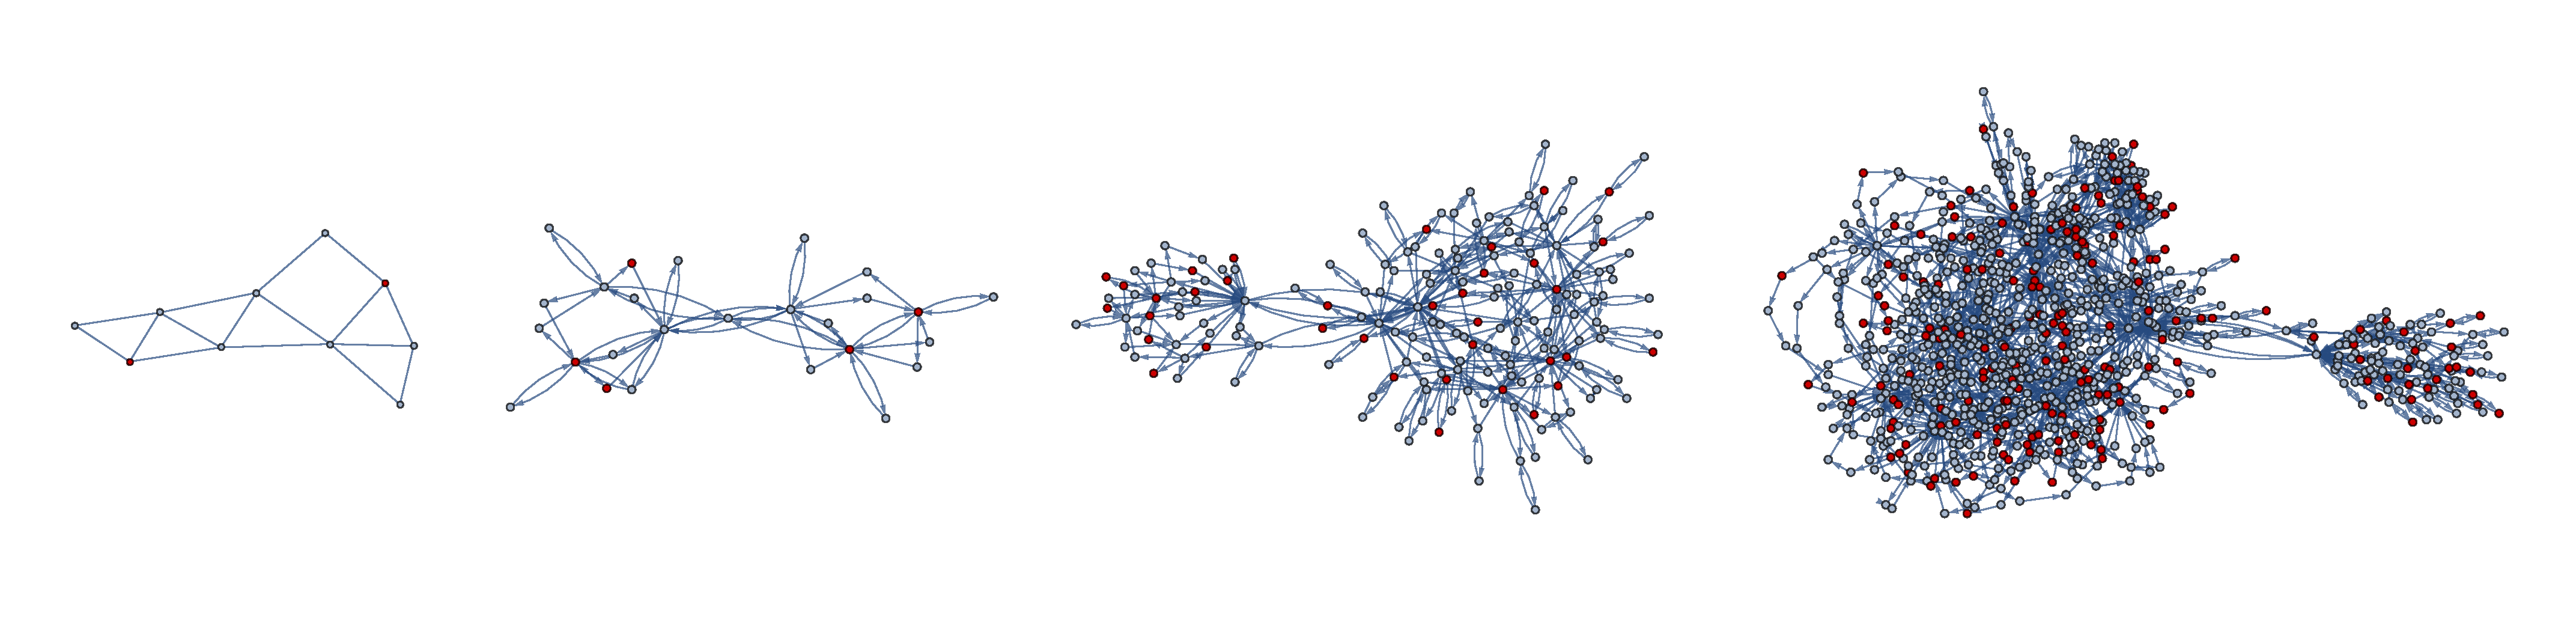
\includegraphics[scale=0.21]{images/synchspecexample.pdf}
    \caption{A sequence of specializations is shown where at each step the graph is specialized over a random subset consisting of twenty percent of its vertices shown in red. The result is a graph that has many real-world like features; a right-skewed degree distribution, is disassociative by degree, has a modular and hierarchical topology, and has the {small world property}.}
    \label{fig:trafficexample001}
\end{figure}

It is worth mentioning that the specialization model presented here is a simplified version of the model introduced in \cite{8} in that we limit the sets we specialize to connected subgraphs.
However, the statistical features as well as spectral and dynamic results established in \cite{8,Bunimovich20} still hold, as the method of specialization described here can be adapted to the method
described in \cite{8,Bunimovich20}.
In that sense, this method is more general.

\section{Dynamical Network Specialization}
To understand how specialization affects the dynamics of a network we need a way to specialize a dynamical network $(F,X)$. We do this by specializing the network's adjacency matrix $A$ (see Definition~\ref{def:dn}).
Here we rely on the fact that the matrix $A$ describes the underlying graph structure of the network.
To specialize the matrix $A$ we simply specialize the associated graph of interactions $G$ where $A=A(G)$.

%The adjacency matrix of the resulting graph is the specialized matrix. This specialization of a matrix in terms of a graph is possible as there is a one-to-one relation between a graph $G=(V,E)$ and its adjacency matrix $A(G)\in\mathbb{R}^{n\times n}$.

\begin{definition}\label{def:matspec}\textbf{(Matrix Specialization)}
Let $A\in\{0,1\}^{n\times n}$ be the adjacency matrix of the graph $G=(V,E)$ and suppose $S\subseteq V$.
We define the adjacency matrix of the specialized graph $\bar{G}=\bar{G}(S)$ to be the matrix $\bar{A}=\bar{A}(S)\in\{0,1\}^{m\times m}$, which we call the {specialization} of the matrix $A$ over $S$.
For $\bar{G}=(\bar{V},\bar{E})$, if the vertex $j\in\bar{V}$ is a copy of the vertex $i\in V$ then we say the index $j\in\{1,2,\dots,m\}$ is a {copy} of the index $i\in\{1,2,\dots,n\}$.
\end{definition}

In order to examine network dynamics after specialization, we must establish how the specialized dynamical network inherits the functions $H_{ij}:\R \to \R$.
These functions describe the influence element $j$ has on element $i$ in the original network.
To define this process of inheritance we will use the notion of an origination function.  

\begin{definition}\label{def:orig}\textbf{(Origination Function)}
Suppose $\bar{A}=\bar{A}(S)\in\{0,1\}^{m\times m}$ is a specialization of the matrix $A\in\{0,1\}^{n\times n}$.
Let 
\begin{align*}
    \tau:\{1,2,\dots,m\}\rightarrow \{1,2,\dots,n\}
\end{align*}
be the function where $\tau(j)=i$ if the index $j$ is a copy of the index $i$.
If $j$ is not a copy of any index $i$ then $\tau(j)=j$.
We refer to $\tau$ as the {origination function} of the specialization.
\end{definition}

The origination function describes where an index (vertex) $j$ in a specialized matrix (graph) {originated}.
If $j$ is a copy of $i$ then $\tau(j)=i$ or the index (vertex) $j$ was originally the index (vertex) $i$ before the matrix (graph) was specialized.
This gives us an equivalence relation where indices (vertices) are in the same class if they are copies of the same index (vertex).
Specifically, two indices (vertices) $i$ and $j$ are {copies of the same index (vertex)} if $\tau(i)=\tau(j)$.

The origination function allows us to define the specialization of the dynamical network $(F,\mathbb{R}^n)$.

\begin{definition}\label{def:specdyn}\textbf{(Specialization of Dynamical Networks)} 
Suppose $(F,\mathbb{R}^n)$ is a dynamical network given by Equation \eqref{eq:netclass}.
If $S\subseteq \{1,2,\dots,n\}$ then the {specialization} of $(F,\mathbb{R}^n)$ over $S$ is the dynamical network $(\bar{F},\mathbb{R}^m)$ where the function $\bar{F}:\mathbb{R}^m\rightarrow\mathbb{R}^m$ has components
\begin{align*}
    \bar{F}_i(\mathbf{y})=\sum_{j=1}^m \bar{A}_{ij}H_{\tau(i)\tau(j)}(y_j) \quad \text{for} \quad i\in \{1,2,\dots,m\}.
\end{align*}
%Here $\bar{A}=\bar{A}(S)\in\{0,1\}^{m\times m}$ and $\tau:\{1,2,\dots,m\}\rightarrow \{1,2,\dots,n\}$ is the origination function of the specialization of the adjacency matrix $A\in\mathbb{R}^{n\times n}$ of $(F,\mathbb{R}^n)$.
\end{definition}


\begin{figure}
    \begin{center}
        \begin{tabular}{cc}
        \hspace{2cm}
        \begin{overpic}[scale=0.25]{images/Specialization10.pdf}
        \put(-9,4){(a) Original Dynamical Network}
        \put(61,4){(b) Specialized Dynamical Network}
        \put(-2,27.75){\tiny{$1$}}
        \put(33.5,27.75){\tiny{$4$}}
        \put(15.75,37.5){\tiny{$2$}}
        \put(15.75,17.5){\tiny{$3$}}
        
        \put(68.5,27.75){\tiny{$1$}}
        \put(100.5,27.75){\tiny{$4$}}
        
        \put(91.5,45){\tiny{$3.1$}}
        \put(87,36.5){\tiny{$2.2$}}
        \put(87,19){\tiny{$3.3$}}
        \put(91.5,10){\tiny{$2.4$}}
        
        \put(75.5,45){\tiny{$2.1$}}
        \put(87,40.5){\tiny{$3.2$}}
        \put(87,14.75){\tiny{$2.3$}}
        \put(75.5,10){\tiny{$3.4$}}
        \end{overpic} &\\
        \hspace{-5cm}
        \begin{overpic}[scale=0.4]{images/ex:sync1.pdf}
        \put(-3,-3){(c) Dynamics of the Original Network}
        \end{overpic} &
        \hspace{-5cm}
        \begin{overpic}[scale=0.4]{images/ex:sync2.pdf}
        \put(6,-3){(d) Dynamics of the Specialized Network}
        \end{overpic}
    \end{tabular}
    \vspace{0.05cm}
    \caption{
        The graph of interactions of the dynamical network $(F,\mathbb{R}^4)$ from Example~\ref{ex:spec} is shown in (a).
        The graph of interactions of the specialized network $(\bar{F},\mathbb{R}^{10})$ of $(F,\mathbb{R}^4)$ over $S=\{2,3\}$ is shown in (b). Copies of vertex 2 from (a) are indicated by 2.1, 2.2, etc. in (b) and the same convention is used for vertex 3.
        In both graphs {self-loops} are omitted, i.e. edges that begin and end at the same vertex. The dynamics of $(F,\mathbb{R}^4)$ is shown in (c). The dynamics of the specialized network $(\bar{F},\mathbb{R}^{10})$ is shown in (d).
        }\label{fig:spec_ex}
    \end{center}
\end{figure}

\begin{example}\label{ex:spec}
Consider the dynamical network $(F,\mathbb{R}^4)$ given by
\begin{align*}
    F\left(\begin{bmatrix}
    x_1 \\
    x_2 \\
    x_3 \\
    x_4
    \end{bmatrix}\right)
    =
    \begin{bmatrix}
    \frac{3}{5}x_1 + t(x_4) + 2 \\
    \frac{9}{10}x_2 + s(x_1) + s(x_3) + \frac{5}{4} \\
     \frac{9}{10}x_3-2t(x_1) + s(x_2) + \frac{7}{4} \\
     \frac{9}{10}x_4-2t(x_2) + s(x_3) + \frac{1}{4}
    \end{bmatrix},  
\end{align*}
where $t(x)=\tanh(x)$ and $s(x)=(1+ e^{-x})^{-1}$.
The graph of interactions of this dynamical network is shown in Figure~\ref{fig:spec_ex}(a).
Choosing $S=\{2,3\}$ results in the specialized dynamical network  $(\bar{F},\mathbb{R}^{10})$ given by
\begin{align*}
    \bar{F}\left(\begin{bmatrix}
    x_1 \\
    x_{2.1} \\
    x_{2.2} \\
    x_{2.3} \\
    x_{2.4} \\
    x_{3.1} \\
    x_{3.2} \\
    x_{3.3} \\
    x_{3.4} \\
    x_4
    \end{bmatrix}\right)
    =
    \begin{bmatrix}
    \frac{3}{5}x_1 + t(x_4) + 2\\
    \frac{9}{10}x_{2.1} + s(x_1) + s(x_{3.1}) + \frac{5}{4} \\
    \frac{9}{10}x_{2.2} + s(x_1) + s(x_{3.2}) + \frac{5}{4} \\
    \frac{9}{10}x_{2.3} + s(x_{3.3}) + \frac{5}{4} \\
    \frac{9}{10}x_{2.4} + s(x_{3.4}) + \frac{5}{4} \\
    \frac{9}{10}x_{3.1} + s(x_{2.1}) + \frac{7}{4} \\
    \frac{9}{10}x_{3.2} + s(x_{2.2}) + \frac{7}{4} \\
    \frac{9}{10}x_{3.3} - 2t(x_1) + s(x_{2.3}) + \frac{7}{4} \\
    \frac{9}{10}x_{3.4} - 2t(x_1) + s(x_{2.4}) + \frac{7}{4} \\
    \frac{9}{10}x_4 - 2t(x_{2.2}) - 2t(x_{2.4}) + s(x_{3.1})  + s(x_{3.3}) + \frac{1}{4}
    \end{bmatrix}.
\end{align*}
The specialized network's graph of interactions is shown in Figure~\ref{fig:spec_ex}(b) where the vertices  2.1, 2.2, 2.3, and 2.4 are copies of vertex 2 shown in (a).
The same convention is used for vertex 3.

In this example the original unspecialized network $(F,\mathbb{R}^4)$ has a globally attracting fixed point $\mathbf{x}^*\in\mathbb{R}^4$ shown in Figure~\ref{fig:spec_ex}(c).
The specialized network $(\bar{F},\mathbb{R}^{10})$ also has a globally attracting fixed point $\bar{\mathbf{x}}^*\in\mathbb{R}^{10}$ shown in Figure~\ref{fig:spec_ex}(d).
The difference between the two fixed points is that each component of $\mathbf{x}^*$ is unique whereas in $\bar{\mathbf{x}}^*$ the components $\bar{x}_{2.1}^*=\bar{x}_{2.2}^*$, $\bar{x}_{2.3}^*=\bar{x}_{2.4}^*$, $\bar{x}_{3.1}^*=\bar{x}_{3.2}^*$, and $\bar{x}_{3.3}^*=\bar{x}_{3.4}^*$.
That is, the dynamics of these pairs of network elements {synchronize asymptotically}.
\end{example}

Here we note that this synchronization phenomenon occurs between components that are copies of the same vertex.
However, not all copies of the same component synchronize.
To understand how and when specialization leads to synchronization we need to understand the specific graph structures that occur via specialization.
This is the main focus of the following section.


\chapter{Equitable Partitions on Graphs and Specialized Graphs}\label{chapt:eqp}

\section{Equitable Partitions}

To understand what causes the synchronization found in Example~\ref{ex:spec}, we need to understand the structures that are created by network specialization.
The structures we consider are known as equitable partitions, which have been shown to be a necessary condition for network synchronization \cite{11}.
While equitable partitions are typically defined for undirected graphs, we extend the standard definition of an equitable partition to be applicable to the directed graphs we consider in this paper \cite{Godsil01}.

\begin{definition}\label{def:ep}\textbf{(Equitable Partition)}
Let $G=(V,E)$ with adjacency matrix $A=A(G)$.
A partition $\pi=\{V_1,V_2,\dots,V_k\}$ of the vertices $V$ is an equitable partition if the sum
\begin{equation}\label{eq:ep}
    \sum_{j\in V_b}A_{ij}=D_{ab}    
\end{equation}
is constant for any $i\in V_a$.
The matrix $D\in\mathbb{N}^{k\times k}$ is called the {divisor matrix} of $A$ associated with $\pi$. 
\end{definition}

For undirected graphs, a partition $\pi=\{V_1,V_2,\dots,V_k\}$ is a partition in which every vertex in $V_i$ is adjacent to the same number of vertices in $V_j$ for all $i$ and $j$.
In Definition~\ref{def:ep} the notion of an equitable partition is generalized to directed graphs.
By definition \ref{def:ep} every vertex in $V_i$ had the same number of incoming edges from vertices in $V_j$ for all $i$ and $j$.
This is an extension of the notion of an equitable partition to directed graphs since any undirected graph that satisfies Definition~\ref{def:ep} satisfies the original definition of an equitable partition.
It is equivalent to the notion of an equitable receiving partition in \cite{Lund21}.
We define the equitable partition in this way because we ultimately care about network dynamics, and a component's dynamics depends on the components that have an influence on it, i.e. on the incoming edges.

\begin{example}\label{ex:create-eqp}
Consider the graph $G$ in Figure~\ref{fig:trafficexample5} (left).
This graph has only the {trivial} equitable partition in which each vertex is in its own partition element.
If the graph is specialized over the two central vertices as in Figure~\ref{fig:trafficexample2} the result is the graph $\bar{G}$ shown on the right.
This graph has the nontrivial equitable partition consisting of two yellow, two purple, two green, and two orange vertices, where each of the other vertices are in their own partition element.  
\end{example}

\begin{figure}
\begin{center}
    \begin{tabular}{c}
    \begin{overpic}[scale=0.33]{images/SynchSpecFig2.pdf}
    \put(23,3){$G$}
    \put(77,3){$\bar{G}$}
    \end{overpic}
\end{tabular}
\caption{
    The graph $G$, shown left, is specialized as in Figure~\ref{fig:trafficexample2}.
    The result is the graph $\bar{G}$, shown right.
    The graph $G$ has only the trivial equitable partition.
    The specialized graph $\bar{G}$ has the equitable partition consisting of the two yellow, two purple, two green, and two orange vertices, where each of the other vertices, shown in blue, are in their own partition element consisting of a single vertex.
    }\label{fig:trafficexample5}
\end{center}
\end{figure}

% \begin{remark} \textbf{(Network Communities)}\label{rem:coms}
% We can interpret the elements of an equitable partition as network communities. However, such communities are not the communities that are typically defined in network science. Most often such communities are defined as highly {modular} subnetworks, meaning that there are very few connections between different communities and many connections between members of the same community. In Figure~\ref{fig:trafficexample5} (right) the communities formed from equitable partitions have no interconnections and are in this sense very different from standard communities.

% %One example that may clarify this conception of community could be found in a wireless internet network. Consider the local network in a home or office, where there is a single large router, connected to several WiFi ranges extenders, these range extenders then each service several different devices. Conceptually, we expect all of the range extenders to be in the same community, as defined by the equitable partition. Rigorously, this would only hold if each range extender is connected to the same number of devices, but this is not an unrealistic condition. In this more rigorous case, we would also have that all of the devices are in the same community, despite the average degree of the network restricted to that community is 0 (the total degree is also 0 in this case).
% \end{remark}

%There are often many potential partitions of a graph $G$ that are equitable. One that will be our main focus is the {coarsest equitable partition}, which is a unique equitable partition with the smallest number of partition elements (see \cite{Sidd18}). 

%\begin{example}
%The graph $G$ shown in Figure~\ref{fig:trafficexample6}, both left and right, is shown with two different equitable partitions. The one on the left is the graph's coarsest equitable partition having two elements (colors). The equitable partition on the right is a refinement of the one on the left having three partition elements (colors). 
%\end{example}

To understand why the synchronization that appears in specialized networks is not just the synchronization of copies of the same vertex we need to consider the notion of an {in-branch}, which is defined as follows.

\begin{definition}\label{def:inout}\textbf{(In-Branches)}
Let $G=(V,E)$ be a graph and $S\subseteq V$.
For the branch $\beta = \{i,e_{ik},G_S,e_{\ell j},j\}$ let $\beta^{in}=\{i,e_{ik},G_S\}$
be the {in-branch} of $\beta$.
The in-branches  
\begin{align*}
    \bar{\gamma}^{in}=\{i,e_{i\bar{p}},G_S(\gamma)\} \quad \text{and} \quad \bar{\delta}^{in}=\{i,e_{i\bar{q}},G_S(\delta)\}
\end{align*}
of the specialized graph $\bar{G}=\bar{G}(S)$ are {copies} of the in-branch $\beta^{in}$ of $G$ if the vertices $\bar{p}$ and $\bar{q}$ are copies of the same vertex $k$.
Two vertices $v\in\bar{\gamma}^{in}$ and $w\in\bar{\delta}^{in}$ are said to have the same in-branch if $\bar{\gamma}^{in}$ and $\bar{\delta}^{in}$ are copies of the same in-branch.
\end{definition}

%\begin{figure}
%\begin{center}
%    \begin{tabular}{c}
%    \begin{overpic}[scale=0.45]{SynchSpecFig3.pdf}
%    \put(23,3){$G$}
%    \put(77,3){$G$}
%    \end{overpic}
%\end{tabular}
%\caption{Left: The coarsest equitable partition of the %graph $G$ consisting of two elements shown as red and %yellow vertices, respectively. Right: A refinement of this %partition is the equitable partition with three elements %shown as the red, yellow, and green vertices, %respectively.}\label{fig:trafficexample6}
%\end{center}
%\end{figure}

While no two branches $\bar{\gamma},\bar{\beta}$ in $\bar{G}$ are copies of the same branch in the sense of Definition~\ref{def:inout}, there are potentially many in-branches that are copies of the same in-branch.
For instance, in the specialized graph $\bar{G}$ in Figure~\ref{fig:trafficexample5} (right) the two top branches with yellow and purple vertices have in-branches that are copies of the same in-branch.
The bottom two branches with orange and green vertices also have in-branches that are copies of the same in-branch. 

\section{Creation and Preservation of Equitable Partitons}

The notion of two vertices being from the same in-branch allows us to give the following result regarding the way specialization creates equitable partitions.

\begin{theorem}{\textbf{(Emergence of Equitable Partitions via Specialization)}}\label{thm:coarse}
Let $\bar{G}=(\bar{V},\bar{E})$ be a specialization of the graph $G$.
Then $\bar{G}$ has an equitable partition $\bar{\pi}$ where vertices that are\\
(i) copies of the same vertex; and\\
(ii) have the same in-branch;\\
belong to the same element of $\bar{\pi}$.
\end{theorem}

\begin{proof}
Let $A$ be the adjacency matrix of $G=(V,E)$ and $\bar{A}$ the adjacency matrix of the specialized graph $\bar{G}=(\bar{V},\bar{E})$.
Suppose all vertices that satisfy conditions (i) and (ii) are in the same element of $\bar{\pi}=\{\bar{V}_1,\bar{V}_2,\dots,\bar{V}_k\}$ and all other vertices are in their own element of $\bar{\pi}$.
Then each element $\bar{V}_a\in\bar{\pi}$ is either a single vertex in the {complement} $S^c$ of $S$ or is comprised of copies of the same vertex, each with the same in-branch. 

If $\bar{V}_a\in\bar{\pi}$ consist of single vertex in $S^c$ then Equation \eqref{eq:ep} holds trivially.
Suppose then that the partition element $\bar{V}_a$ has the property that (i) each of its vertices are copies of the same vertex and (ii) each vertex has the same in-branch.
If $\bar{V}_b=\{b\}$ is a single vertex in $S^c$ then for any $i,j\in\bar{V}_a$
\begin{align*}
    \sum_{\ell\in \bar{V}_b}\bar{A}_{i\ell}=\bar{A}_{ib}=A_{\tau(i)\tau(b)}=A_{\tau(j)\tau(b)}=\bar{A}_{jb}=\sum_{\ell\in \bar{V}_b}\bar{A}_{j\ell}
\end{align*}
where the third equality follows from the fact that all vertices in $\bar{V}_a$ are copies of the same vertex, i.e. $\tau(i)=\tau(j)$. Since $i,j\in\bar{V}_a$ are arbitrary Equation \eqref{eq:ep} holds in this case. 

If $\bar{V}_b$ is not a single vertex in $S^c$ then all vertices in $\bar{V}_b$ are copies of the same vertex with the same in-branch.
In this case, if $\alpha\in\bar{V}_a$ there is a branch $\beta_\alpha$ such that $\alpha\in G_S(\beta_\alpha)$ is in $\bar{G}$ in which there is exactly one element $b_\alpha\in\bar{V}_b$.
The reason is that there is exactly one copy of each vertex of $G_S$ in each copy of $G_S$ implying $\sum_{b_\ell\in\bar{V}_b} \bar{A}_{\alpha b_\ell}=\bar{A}_{\alpha b_\alpha}$.
Thus, for any $i,j\in\bar{V}_a$ where $i\in\bar{\beta}_i^{in}$ and $j\in\bar{\beta}_j^{in}$ we have
\begin{align*}
    \sum_{b_\ell\in\bar{V}_b}\bar{A}_{ib_\ell} = \bar{A}_{i b_i} = A_{\tau(i)\tau(b_i)} = A_{\tau(j)\tau(b_j)} = \bar{A}_{jb_j} = \sum_{b_\ell\in\bar{V}_b}\bar{A}_{jb_\ell}.
\end{align*}
where the third equality holds as all vertices in $\bar{V}_a$ and $\bar{V}_b$ are copies of the same vertices, respectively.
Again as $i,j\in\bar{V}_a$ are arbitrary Equation \eqref{eq:ep} holds in this case. 

It, therefore, follows that $\bar{\pi}$ is an equitable partition of $\bar{G}$.
\end{proof}

\begin{example}
Consider the specialized graph $\bar{G}$ shown in Figure \ref{fig:trafficexample5} (right).
The two yellow vertices in $\bar{G}$ are (i) copies of the left vertex that is specialized in $G$ and (ii) have the same in-branch.
Therefore these vertices can be put into the same element of the equitable partition $\bar{\pi}$.
Similarly, the purple, green, and orange vertices can be put in the same partition element, respectively.
We note that the green and yellow (orange and purple) vertices cannot be put into the same element of $\bar{\pi}$ although these are copies of the same vertex.
\end{example}

An equitable partition divides up a network into what could be considered communities.
However, {communities} are typically defined to be highly interconnected subgroups of vertices with relatively few connections to other communities \cite{Newman10}.
In contrast, equitable partitions cut across highly connected subsets of a network so that members of the same partition element belong to what can be considered different communities (cf. Figure \ref{fig:trafficexample5} (right)).
However, members of the same cluster have a similar {role} in their respective communities both in terms of their position in their community and dynamics (see Theorem \ref{thm:sync_and_eqp}).

As members of the same element of an equitable partition often are influenced by and influence the same type and number of other components, each member has what could be considered the same {role} within their own community.

%Many networks roles are clearly defined within communities; experts and influences in social networks, binding and nonbinding proteins in bioregulatory networks, and director, actors, grips, etc. in the professional network of film crews. Specialization not only creates communities, by isolating copies of $G_S$, it also specifies roles within these communities which are given by the elements of the equitable partition $\bar{\pi}$ described in Theorem \ref{thm:coarse}. This notion of role is later reinforced in Section \ref{sec:4} where we describe how components in the same element of $\bar{\pi}$ can synchronize (see Theorem \ref{thm:sync_and_eqp}). 

We note that not only do we have the creation of non-trivial equitable partitions within specialized graphs, specialization can also preserve equitable partitions.
To describe this we require the following definition.  

\begin{definition}\textbf{(Partition Respecting Maps)}
Let $G=(V,E)$ be a graph with an equitable partition $\pi=\{V_1,\dots,V_k\}$.
For $A,B\subseteq V$ the function $f:A\to B$ {respects} the partition $\pi$ if it is bijective and for each $a\in A$ with $a\in V_i$ we have $f(a)\in V_i$.
\end{definition}

This allows us to prove the following result describing how a graph's equitable partition can be preserved under specialization.

% \begin{theorem}{\textbf{(Partition Conservation Under Specialization)}}\label{thm:part_conv}
% Suppose $G=(V,E)$ has the equitable partition $\pi=\{V_1,V_2,\dots,V_k\}$. If $G$ is specialized over the set $S=\cup_{i\in\mathcal{I}}V_i$ for some subset $\mathcal{I}\subseteq\{1,2,\dots,k\}$ then $\bar{G}=(\bar{V},\bar{E})$ has an equitable partition $\bar{\pi}$ where all elements $A\in\bar{\pi}$ are either:\\
% (1) a set of specialized vertices where for any $a,b\in A$, $\tau(a),\tau(b)\in V_{\ell}\in\pi$ and there exists a function from the in-branch of $a$ to the in branch of $b$ that respects $\pi$,\\
% (2) or $V=V_i\in\pi$ where $i\notin\mathcal{I}$.
% \end{theorem}

\begin{theorem}{\textbf{(Partition Conservation Under Specialization)}}\label{thm:part_conv}
Suppose $G=(V,E)$ has the equitable partition $\pi=\{V_1,V_2,\dots,V_k\}$.
If $G$ is specialized over the set $S=\cup_{i\in\mathcal{I}}V_i$ for some subset $\mathcal{I}\subseteq\{1,2,\dots,k\}$ then $\bar{G}=(\bar{V},\bar{E})$ has an equitable partition $\bar{\pi}=\{\bar{V}_1,\bar{V}_2,\dots,\bar{V}_\ell\}$ where any partition element $\bar{V}_j\in\bar{\pi}$ is either:\\
(1) a set of specialized vertices such that for any $a,b\in \bar{V}_j$ the vertices $\tau(a),\tau(b)$ are elements of some $V_{i}\in\pi$ for $i\in\mathcal{I}$ and there exists a function from the in-branch of $\tau(a)$ to the in-branch of $\tau(b)$ that respects $\pi$; or\\
(2) $\bar{V}_j=V_i\in\pi$ where $i\notin\mathcal{I}$.
\end{theorem}

Before proving Theorem \ref{thm:part_conv} we note that the equitable partition $\bar{\pi}$ described in this theorem contains two kinds of elements.
The first kind are those that contain specialized vertices.
The second kind are elements that consist of the unspecialized elements found in $\pi$.
The fact that these elements survive the specialization process means that we can, at least partially, preserve the equitable partition $\pi$ by specializing over subsets of its elements (see Example \ref{ex:thm2}).
We now give a proof of Theorem \ref{thm:part_conv}.

\begin{proof}
Let $a,b\in V_i\subset S$.
We first show inductively that there exists a $\pi$ respecting map between an in-branch of $a$ and an in-branch of $b$.
Suppose that $a$ has a neighbor that is not in $S$.
By the construction of $S$, vertex $b$ must also have a neighbor not in $S$ that is in the same element of $\pi$.
If $a$ has no such neighbor then we may simply choose a neighbor and repeat the procedure, eventually arriving at a vertex that is not in $S$ via some path $p_a$.
Because $a$ and $b$ are in the same element of $\pi$, we can similarly find a path $p_b$ analogous to $p_a$ starting at $b$, which allows us to define a $\pi$ respecting map for $a$ and $b$.
%There are certain trivial cases where the component containing $a$ is disconnected from the rest of the graph, in which case the component containing $b$ is also disconnected. These cases do not effect our results.

With this in place, consider an element $\bar{V}_i\in\bar{\pi}$ of the first kind, described by (1) in Theorem \ref{thm:part_conv}, and let $a,b\in \bar{V}_i$.
If $\bar{V}_j$ is another element of $\bar{\pi}$ we have two cases. If $\bar{V}_j$ is of the first kind then it contains only vertices specialized from the original graph $G$.
Therefore, for any element $\ell\in \bar{V}_j$ with $e_{\ell a}\in\bar{E}$ there must be {an} edge $e_{\tau(\ell)\tau(a)}\in E$.
Because $\tau(a)$ and $\tau(b)$ are in the same element of $\pi$ it must be the case that there is some other vertex $c\in V$ in the same element of $\pi$ as $\tau(\ell)$ with $e_{c\tau(b)}\in\bar{E}$.
Since $\tau(\ell)$ and $c$ are both in the same element of $\pi$ there must then exist a $\pi$ respecting map between an in-branch of $\tau(\ell)$ and $c$.
Therefore there is a copy $\bar{c}$ of $c$ that is in $\bar{V}_j$, and it follows that 
\begin{align*}
    \sum_{\ell\in \bar{V}_j}\bar{A}_{a\ell} = \sum_{\ell\in \bar{V}_j}\bar{A}_{b\ell},
\end{align*}
% If $\tau(\ell)$ is in the in-branch of $\tau(a)$ then there must exist a vertex $c$ in the in branch of $\tau(b)$ with $c$ in the same element of $\pi$ as $\tau(\ell)$ because of the $\pi$ respecting map between the in-branches of $\tau(a)$ and $\tau(b)$. In this case we have that there must exist a copy $\bar{c}$ of $c$ that is in $\bar{V}_j$ as $c$ and $\tau(\ell)$ are in the same element of $\pi$ and the partition respecting map between the in-branches of $\tau(a)$ and $\tau(b)$ also defines a map between the in branches of $\tau(\ell)$ and $c$.
% Finally there must also be some copy $\bar{c}$ of $c$ in the specialized branch containing $b$ with an accompanying edge $e_{\bar{c} b}$. We can claim that $\bar{c}\in \bar{V}_j$ by considering the $\pi$ respecting map. If $\ell$ is in the in-branch of $a$, then we may choose $c$ so that $\bar{c}$ is in the in-branch of $b$, in this case we use a restriction of the $\pi$ respecting map to argue that $\bar{c}$ and $\ell$ are in the same element. If $\ell$ is not in the in-branch of $a$ then we extend the $\pi$ respecting map to include $a$ and $b$ to argue that $\bar{c}$ and $\ell$ are in the same element. So we have
where $\bar{A}$ is the adjacency matrix of $\bar{G}$.

If instead $\bar{V}_j$ is of the second kind, described by (2) in Theorem \ref{thm:part_conv}, then we rely on the $\pi$ respecting map. For every $k\in \bar{V}_j$ with an edge $e_{ka}$ there exists an $\ell\in \bar{V}_j$ with an edge $e_{\ell a}$.
Therefore we have 
\begin{align*}
    \sum_{\ell\in \bar{V}_j}\bar{A}_{a\ell} = \sum_{\ell\in \bar{V}_j}\bar{A}_{b\ell},
\end{align*}
in this case as well.

The last case to consider is if $\bar{V}_i\in\bar{\pi}$ is of the second kind, i.e. $\bar{V}_i = V_m\in\pi$ for some $m\notin\mathcal{I}$.
As before let $a,b\in\bar{V}_i$ and suppose $\bar{V}_j$ is another element of $\bar{\pi}$ for $j\notin\mathcal{I}$.
Then for any $c\in\bar{V}_j$ with an edge $e_{ca}\in\bar{E}$ there must also be an edge $e_{db}\in\bar{E}$ for $d\in \bar{V}_j$ since none of the vertices in $\bar{V}_{j}$ have changed when $G$ was specialized.

If $\bar{V}_j\in\bar{\pi}$ is of the first kind then $c\in\bar{V}_j$ is a specialized vertex.
Then, if there is an edge $e_{ca}\in\bar{E}$ it follows that as $c$ is a copy of $\tau(c)\in V_{k}\in\pi$ there is an edge $e_{\tau(c)a}\in E$.
Since $a,b$ are both in $V_m\in\pi$ there is a vertex $d\in V_{k}$ with $e_{db}\in E$.
Since $d$ and $\tau(c)$ are both in $V_{k}$ there must be some in-branch of $d$ that satisfies the $\pi$ respecting map criterion.
There is then a copy $\bar{d}\in\bar{V}$ of $d$ that is in the same element of $\bar{\pi}$ as $c$, and therefore we have the existence of an edge $e_{\bar{d}b}$ where $c,\bar{d}\in \bar{V}_{\ell}\in\bar{\pi}$.
It then follows that $\bar{\pi}$ is an equitable partition of the specialized graph $\bar{G}$.
\end{proof}

\begin{figure}
\begin{center}
    \begin{tabular}{c}
    \begin{overpic}[scale=0.36]{images/SynchFigEP.pdf}
    \put(23,0.5){$G$}
    \put(77,0.5){$\bar{G}$}
    \put(72.5,21){$a$}
    \put(80.5,3.5){$b$}
    \put(10,19){$u$}
    \put(35,6){$v$}
    \put(16.5,15){$\tau(a)$}
    \put(25,15){$\tau(b)$}
    \end{overpic}
\end{tabular}
\caption{
    The graph $G$, shown left, has the equitable partition consisting of the four sets of red, yellow, green, and brown vertices.
    Specializing $G$ over the red vertex set $S$ results in the graph $\bar{G}=\bar{G}(S)$, shown right.
    The graph $\bar{G}$ has the equitable partition consisting of the fives vertex sets colored yellow, green, brown, orange, and purple, respectively.
    As $S$ is a subset of the partition elements of $G$ then the other partition elements of $G$ are preserved under this specialization (see Theorem \ref{thm:part_conv}.)
    }\label{fig:trafficexample3}
\end{center}
\end{figure}

\begin{example}\label{ex:thm2}
Consider the graph $G$ and its specialization $\bar{G}$ over the red vertices of $G$ shown in Figure \ref{fig:trafficexample3}, which is a slight modification of the graph in Figure \ref{fig:trafficexample5}.
The graph $G$ has the equitable partition $\pi=\{V_1,V_2,V_3,V_4\}$ consisting of the red, yellow, green, and brown vertices, respectively.
When $G$ is specialized over the red vertices $S=V_1$ the resulting graph $\bar{G}$ has the same equitable partition as $G$ when we restrict our attention to the complement $S^c=\cup_{i=2}^4 V_i$ of $S$.
That is, each of $V_2$, $V_3$, and $V_4$ is an element of the equitable partition shown in \ref{fig:trafficexample3} (right) that is preserved under specialization.

Moreover, for any vertices $a$ and $b$ in the same element of $\bar{\pi}$ we can find a partition respecting function from the branch of $\tau(a)$ to the branch of $\tau(b)$.
For instance, for $a$ and $b$ shown in $\bar{G}$ the in-branch of $\tau(a)$ is mapped to the in-branch of $\tau(b)$ in this manner via $f(u)$=v, $f(\tau(a))=\tau(b)$, and $f(\tau(b))=\tau(a)$.
\end{example}

If the specialized set $S$ does not divide an element of a graph's equitable partition the nonspecialized elements of the partition are preserved by Theorem \ref{thm:part_conv}. (We note that the way equitable partitions evolve inside the specialized part of the graph is described by Theorem \ref{thm:coarse}.)  

The main question we consider in the following section is how specialization as a form of network growth effects the dynamics of a network, specifically how equitable partitions form in dynamical networks and how these structures effect the network's dynamics.

\chapter{Specialization and the Emergence of Cluster Synchronization}\label{chapt:sync}
In the previous chapter we related network specialization to the formation of nontrivial equitable partitions.
The question we consider here is can we extend our results from the previous chapter to dynamical networks, and to what extent equitable partitions result in synchronous behavior in dynamical networks.

\section{Equitable Partitions on Dynamical Networks}
As we consider the effects of specialization on dynamical networks we first need a notion of an equitable partition of a dynamical network.

% One can see how this would naturally lead to synchronous behaviour in a dynamical network, and it was the exploration of the synchrony we observed in specialized networks that led us to examine the equitable partition on dynamical networks. This analysis of network synchronization through the lens of equitable partitions is well established by \cite{Sidd18}. In the 2018 paper \cite{Sidd18}, Siddique et. al. demonstrate that equitable partitions define a necessary condition for community synchronization. As implied by the title of this paper, we are examining the relationship that network specialization has with synchronizing communities. The main results of this paper rely on viewing network specialization through the lens of the equitable partition. To begin forming that lens, let us examine the simplest results related to equitable partitions and network specialization.

%The main results of this paper focus on the effects that specialization has on dynamical networks. Specifically, we are interested in the synchrony created in dynamical networks by the process of specialization. This evolution also effects the network's ability to perform its intended function. This function is not only dependent on the network's topology but also on the type of dynamics that emerges from the interactions between the network elements, i.e. the dynamics \emph{on} the network. For instance, power is transferred efficiently in power grids when the grid is synchronized.

%Next we will discuss the effect specialization has on the dynamical stability of copies of strongly connected components within a network. We will consider both the linear and nonlinear cases.

\begin{definition}\textbf{(Equitable Partition of a Dynamical Network)}\label{def:net-eqp}
Let $(F,\mathbb{R}^{n})$ be a dynamical network given by Equation \eqref{eq:netclass}, so that each component $F_i:\mathbb{R}^n\rightarrow\mathbb{R}$ has the form 
\begin{equation}\label{eq:ref}
F_i(\mathbf{x})=\sum_{j=1}^n A_{ij}H_{ij}(x_j) \quad \text{for} \quad i\in\{1,2,\dots,n\}.
\end{equation}
The partition $\pi=\{V_1,V_2,\dots,V_k\}$ of the network elements $\{1,2,\dots,n\}$ is an {equitable partition} if the function    
\begin{equation}\label{eq:DSEP}
f_i(\mathbf{x})=\sum_{j\in V_b}A_{ij}H_{ij}(x_j)
\end{equation}
is the same for every $i\in V_a$ and any partition element $V_b$.
\end{definition}

Note that if $H_{ij}(x_j)=H(x_j)$ for all $i$ and $j$ then the dynamical network $(F,\mathbb{R}^n)$ has an equitable partition $\pi$ if and only if $\pi$ is an equitable partition of the network's graph of interactions.
This is the type of equitable partition considered, for instance, in \cite{11}.
The definition given above is more general as it allows for potentially different functions to combine into the same function $f_i(\mathbf{x})$ for all indices $i$ in some partition element of $\pi$.

% Moreover, this framework also allows us to extend our analysis to {weighted networks}, commonly studied in network science \cite{Newman10}.
% If we choose each $H_{ij}(x_j)=c_{ij}\in\mathbb{R}$ to be a constant then $(F,\mathbb{R}^n)$ can be thought of as a {weighted network} where the edge $e_{ij}$ has weight $c_{ij}$ with equitable partitions of the weighted network are given by Equation \ref{eq:DSEP}.

In Chapter \ref{chapt:eqp} we considered how specialization creates both a community and a role structure.
The natural communities formed by specialization are the specialized subnetworks themselves (see \cite{8}) and the roles within these communities correspond to the elements of the equitable partition that are a result of specialization (cf. Theorem \ref{thm:coarse}).
Here we use the notion of an equitable partition of a dynamical network to show that network components in the same partition element have the potential to have the same dynamics, i.e. the potential to {synchronize} (see Theorem \ref{thm:sync_and_eqp}).
This similarity in dynamics reinforces the idea that equitable partitions are related to role structure within communities.
This type of synchronization is referred to as {cluster synchronization} as vertices in the same partition element, i.e. {cluster}, synchronize.

%The equitable partition associates vertices across different modular subnetworks or communities, therefore using the work community to describe the association defined by an equitable partition is not necessarily appropriate. So, we call the associations formed by the equitable partition \emph{roles}. To illustrate this concept consider a community-like network such as a film crew. Each film crew is its own community, however each member of the film crew has a distinct role: director, actress, grip, etc. and those roles are identifiable across separate film crews. Observationally, we can consider the similar behavior of say directors across multiple film crews to be a form of synchrony. We have shown that specialization tends to create multiple highly modular subnetowrks with nontrivial equitable partitions, as we saw in Figure \ref{fig:trafficexample5}, so in this section we will examine the synchronization that we observe among different roles after specialization.

To describe the dynamic consequences of network specialization we will use the concepts of an attracting fixed point and, more generally, attracting sets.
A point $\mathbf{x}^*\in\mathbb{R}^n$ is a {fixed point} of a dynamical network $(F,\mathbb{R}^n)$ if $F(\mathbf{x}^*)=\mathbf{x}^*.$ The point $\mathbf{x}^*$ is {attracting} if there is an open set $U$ containing $\mathbf{x}^*$ such that {$F(U)\subset U$ and $\cap_{k\geq 0}F^k(U)=\{\mathbf{x}^*\}$}.
The point $\mathbf{x}^*$ is {globally attracting} if $U=\mathbb{R}^n$.
If $\mathbf{x}^*$ is attracting then $\lim_{k\rightarrow\infty}F^k(\mathbf{x}_0)=\mathbf{x}^*$ for any $\mathbf{x}_0\in U$.
This idea of an attracting fixed point can be extended to a network's synchronization manifold.

\begin{definition}\textbf{(Cluster Synchronization in Dynamical Networks)}\label{def:sync}
Let $(F,\mathbb{R}^n)$ be a dynamical network and $\pi=\{V_1,\dots,V_k\}$ a partition of the network elements $\{1,\dots,n\}$.
We define the {synchronizing manifold} of $(F,\mathbb{R}^n)$ with respect to $\pi$ to be the set 
\begin{align*}
    M(\pi) = \left\{\mathbf{x}\in\mathbb{R}^n : x_i=x_j \ \ \text{for all} \ \ i,j\in V_a \ \ \text{and} \ \  a=1,\dots,k\right\}.
\end{align*}
The dynamical network $(F,\mathbb{R}^n)$ synchronizes with respect to $\pi$ if $M(\pi)$ is {forward invariant}, i.e. $F(M(\pi))\subseteq M(\pi)$.
A subset $N(\pi)\subseteq M(\pi)$ is {attracting} if there is an open set $U$ containing $N(\pi)$ such that $F(\bar{U})\subset U$ and $\cap_{k\geq 0}F^k(U)=N(\pi)$. The set is {globally attracting} if $U=\mathbb{R}^n$.
\end{definition}

 %By the definition given in \ref{def:sync}, we can observe that for any partition $\pi$, $M(\pi)$ is an intersection of hyperplanes.
%As a simple example, consider the partition $\pi = \{\{1\},\{2,3,4\},\{5,6\}\}.$
%$M(\pi)$ may be defined as the intersection of hyperplanes as follows
%\begin{align*}
%M(\pi) = \left\{x\in\mathbb{R}^5: x_2 = x_3 \right\} \cap \left\{x\in\mathbb{R}^5: x_3 = x_4 \right\}\cap \left\{x\in\mathbb{R}^5: x_5 = x_6 \right\}.
%\end{align*}
%Hence, since $M(\pi)$ is an intersection of hyperplanes, we have that $M(\pi)$ is isomorphic to $\mathbb{R}^k$ where $k=|\pi|$.

\begin{example}
By the definition given in \ref{def:sync}, we con observe that for any partition $\pi$, $M(\pi)$ is an intersection of hyperplanes.
As a simple example, consider the partition $\pi = \{\{1\},\{2,3,4\},\{5,6\}\}$.
$M(\pi)$ may be defined as the intersection of hyperplanes as follows
\begin{align*}
    M(\pi) = \{x \in \R^5: x_2 = x_3\} \cap \{x\in\R^5 : x_3=x_4\} \cap \{x\in\R^5 : x_5=x_6\}.
\end{align*}
Hence, since $M(\pi)$ is an intersection of hyperplanes, we have that $M(\pi)$ is isomorphic to $R^k$ where $k = |\pi|$.
\end{example}

The points on the manifold $M(\pi)$ are those points at which the individual elements of $\pi$ have the same state, i.e.~are {synchronized}.
The dynamical network synchronizes with respect to $\pi$ if it remains on $M(\pi)$ once it enters $M(\pi)$, which is always the case if $\pi$ is an equitable partition.

\begin{theorem}\textbf{(Cluster Synchronization and Equitable Partitions)}\label{thm:sync_and_eqp}
Suppose the dynamical network $(F,\mathbb{R}^n)$ has the equitable partition $\pi=\{V_1,\dots,V_k\}$.
Then $(F,\mathbb{R}^n)$ synchronizes with respect to $\pi$.
\end{theorem}

\begin{proof}
Suppose $\pi$ is an equitable partition of $(F,\mathbb{R}^n)$ and $\mathbf{x}\in M(\pi)$ where, by way of notation, we let $x_\ell=x_b$ if $\ell\in V_b$.
Then for $i,j\in V_a$ we have 
\begin{align*}
    F_i(\mathbf{x})=\sum_{b=1}^k\left(\sum_{\ell\in V_b}A_{i\ell}H_{i\ell}(x_b)\right) &= \sum_{b=1}^k\left(\sum_{\ell\in V_b}A_{j\ell}H_{j\ell}(x_b)\right) = F_j(\mathbf{x})
\end{align*}
where the second equality holds by Equation \eqref{eq:DSEP}.
Hence, if $\mathbf{x}\in M(\pi)$ then $F(\mathbf{x})\in M(\pi)$ implying $M(\pi)$ is forward invariant.
\end{proof}

In Example \ref{ex:spec} the specialized dynamical network $(\bar{F},\mathbb{R}^{10})$ has the equitable partition
\begin{align*}
\pi = \left\{\{1\},\{2.1,2.2\},\{3.1,3.2\},\{2.3,2.4\},\{3.3,3.4\},\{4\}\right\}.
\end{align*}
By Theorem \ref{thm:sync_and_eqp}, if $\mathbf{x}_0\in M(\pi)$ then any iterate $F^k(\mathbf{x}_0)\in M(\pi)$.
The initial condition $\mathbf{x}_0$ shown in Figure \ref{fig:spec_ex} (bottom right), however, is not on this manifold, yet its trajectory is asymptotic to this set.
The reason is that $M(\pi)$ is globally attracting in this example.

\section{Synchronization as a Result of Specialization}

To determine when specialization results in a (globally) attracting synchronization manifold we need to consider the dynamics of the subnetworks specialized in this process.

\begin{definition}\textbf{(Dynamical Subnetworks)}
For a dynamical network $(F,\mathbb{R}^n)$ with components given by Equation \eqref{eq:ref} suppose $S\subset\{1,\dots,n\}$.
We define the subnetwork $(F_S,\mathbb{R}^{|S|})$ to be the dynamical network with components
\begin{align*}
F_i(\mathbf{x}_S)=\sum_{j\in S}A_{ij}H_{ij}(x_j) \quad \text{for all} \quad i\in S
\end{align*}
where $\mathbf{x}_S$ is the restriction of $\mathbf{x}$ to its components indexed by the elements of $S$.
\end{definition}

\noindent A subnetwork of a dynamical network is effectively a restriction of a network to a subset of its components and the interactions between them.

We note that the notions of specialized vertices of a graph $G$, vertices with the same in-branches, and copies of the subgraph $G_S$ can each be extended to the specialization of dynamical networks.
This allows us to state the following theorem.

\begin{theorem}\textbf{(Specialization and the Emergence of Synchronization)}\label{thm:sync}
Let $(\bar{F},\mathbb{R}^m)$ be the specialization of the dynamical network $(F,\mathbb{R}^n)$ over $S\subset\{1,\dots,n\}$.
Then the following hold:\\ 
(a) The network $(\bar{F},\mathbb{R}^m)$ has the equitable partition $\bar{\pi}$ where the specialized components that are (i) copies of the same component and (ii) have the same in-branch are in the same partition element of $\bar{\pi}$.
All other components are in their own partition element.\\
(b) If $(F,\mathbb{R}^n)$ has the equitable partition $\pi=\{V_1,V_2,\dots,V_k\}$ and $S=\cup_{i\in\mathcal{I}}V_i$ for $\mathcal{I}$ some subset of $\{1,2,\dots,n\}$ then $V_i$ is an element of some equitable partition of $(\bar{F},\mathbb{R}^m)$ for all $i\notin\mathcal{I}$.\\
(c) If the subnetwork $(F_S,\mathbb{R}^{|S|})$ has a (globally) attracting fixed point then the synchronization manifold $M(\bar{\pi})$ of the equitable partition $\bar{\pi}$ in (a) is (globally) attracting.
\end{theorem}

\begin{proof}
Let $\bar{\pi}$ be the partition of $(\bar{F},\mathbb{R}^m)$ satisfying the conditions in (a).
Then by the proof of Theorem \ref{thm:coarse} it follows that $\bar{\pi}$ is an equitable partition of $(\bar{F},\mathbb{R}^m)$ if we replace each $A_{ij}$ by $A_{ij}H_{ij}(x_j)$ and $\bar{A}_{ij}$ by $\bar{A}_{ij}H_{ij}(x_j)$.
Similarly, we can modify the proof for Theorem \ref{thm:part_conv} to prove part (b) by taking the partition described in the proof of this theorem and replacing $\bar{A}_{ij}$ by $\bar{A}_{ij}H_{ij}(x_j)$.

% We begin by defining the relevant equitable partition. Taking the coarsest equitable partition we refine it in the following way. Every vertex that is not a copy generated from specialization is in its own element in the equitable partition. Remaining are the elements which contain only vertices that are copies, these we refine by grouping the vertices according to in-branch, so that each element of the refined equitable partition contains only vertices that are copies of the same vertex and which have the same in-branch, similar to requirements (i) and (ii) in Theorem \ref{thm:coarse}.
% So for every element $V_a$ of $\pi$ the refinement of the coarsest equitable partition, we have that either $V_a$ contains only one element, or $\forall i\in V_a$, $\tau(i) = k$ for some $k\in S$ and $\bar{\beta}_i^{\text{in}}=\beta^{\text{in}}$.

To prove part (c), let $(\bar{F}_{S_i},\mathbb{R}^{|S_i|})$ denote the restriction of $(\bar{F},\mathbb{R}^m)$ to the $i$th copy of the subnetwork $(F_S,\mathbb{R}^{|S|})$ of $(F,\mathbb{R}^n)$. If $(\bar{F}_{S_i},\mathbb{R}^{|S_i|})$ and $(\bar{F}_{S_j},\mathbb{R}^{|S_j|})$ have the same in-branch then for $\theta\in S_i$ and $\vartheta\in S_j$ where $\theta$ and $\vartheta$ index copies of the same component
\begin{align*}
    \left|\mathbf{x}_\theta^{k+1} - \mathbf{x}_\vartheta^{k+1}\right| = \left|\bar{F}_{\theta}(\mathbf{x}^{k}) - \bar{F}_{\vartheta}^k(\mathbf{x}^{k})\right|
    = \left|\sum_{h=1}^m\bar{A}_{\theta h}H_{\tau(\theta)\tau(h)}(x_h^{k}) - \sum_{h=1}^m\bar{A}_{\vartheta h}H_{\tau(\vartheta)\tau(h)}(x_h^{k}) \right|.
\end{align*}
Since the restrictions have the same in-branch then there is a single $\ell\in S^c$ such that 
\begin{align*}
    \left|\mathbf{x}_\theta^{k+1} - \mathbf{x}_\vartheta^{k+1}\right| &= \left| \bar{A}_{\theta \ell}H_{\tau(\theta)\ell}(x_{\ell}^k) + \sum_{h\in S_i}\bar{A}_{\theta h}H_{\tau(\theta)\tau(h)}(x_h^{k}) - \bar{A}_{\vartheta \ell}H_{\tau(\vartheta)\ell}(x_{\ell}^{k}) + \sum_{h\in S_j}\bar{A}_{\vartheta h}H_{\tau(\vartheta)\tau(h)}(x_h^{k}) \right|\\
    &=\left|\sum_{h\in S_i}\bar{A}_{\theta h}H_{\tau(\theta)\tau(h)}(x_h^{k}) - \sum_{h\in S_j}\bar{A}_{\vartheta h}H_{\tau(\vartheta)\tau(h)}(x_h^{k}) \right|\\
    &=\left|\left(\bar{F}_{S_i}(\mathbf{x}_{S_i}^k)\right)_{\theta} - \left(\bar{F}_{S_j}(\mathbf{x}_{S_j}^k)\right)_{\vartheta}\right|.
\end{align*}
As this holds for all $\theta\in S_i$, $\vartheta\in S_j$, and both $(\bar{F}_{S_i},\mathbb{R}^{|S_i|})$ and $(\bar{F}_{S_j},\mathbb{R}^{|S_j|})$ are copies of $(F_{S},\mathbb{R}^{|S|})$ then 
\begin{align*}
    \left|\mathbf{x}_{S_i}^{k+1} - \mathbf{x}_{S_j}^{k+1}\right| = \left|\bar{F}_{S_i}(\mathbf{x}_{S_i}^k) - \bar{F}_{S_j}(\mathbf{x}_{S_j}^k)\right| = \left|F_{S}(\mathbf{y}^k) - F_{S}(\mathbf{z}^k)\right|
\end{align*}
where $\mathbf{y}=\mathbf{x}_{S_i}^k$ and $\mathbf{z}=\mathbf{x}_{S_j}^k$.

Suppose $(F_{S},\mathbb{R}^{|S|})$ has an attracting fixed point.
That is, there exists an $\mathbf{x}^*$ and an open set $U\subseteq\mathbb{R}^{|S|}$ with $\bar{F}_S(\bar{U})\subset U$ such that for all {$\mathbf{x}\in U$ the $\lim_{k\rightarrow\infty}F_S^k(\mathbf{x})=\mathbf{x}^*$}. Then for all $\mathbf{y},\mathbf{z}\in U$ we have 
\begin{equation}\label{eq:last}
\lim_{k\rightarrow\infty}\left|\mathbf{x}_{S_i}^{k+1} - \mathbf{x}_{S_j}^{k+1}\right| = \lim_{k\rightarrow\infty}\left|F_{S}(\mathbf{y}^k) - F_{S}(\mathbf{z}^k)\right|=|\mathbf{x}^*-\mathbf{x}^*|=0.
\end{equation}
Since this is true for every pair of restrictions $(\bar{F}_{S_i},\mathbb{R}^{|S_i|})$ and $(\bar{F}_{S_j},\mathbb{R}^{|S_j|})$ that have the same in-branch, the open set $W=(\oplus_{i=1}^N U)\oplus\mathbb{R}^M\subseteq\mathbb{R}^m$ contains a subset $L(\bar{\pi})\subseteq M(\bar{\pi})$ and $\bar{F}(\bar{W})\subset W$ where $N$ is the number of branches in the specialized network and $M$ the number of unspecialized components.
It follows from Equation \eqref{eq:last} that $\cap_{k\rightarrow\infty}F^k(\bar{W}) \subseteq L(\pi)$.
If the fixed point $\mathbf{x}^*$ is globally attracting then $U=\mathbb{R}^{|S|}$ implying $W=\mathbb{R}^m$ so that the equitable partition $\bar{\pi}$ is globally attracting, completing the proof.
\end{proof}

Parts (a) and (b) of Theorem \ref{thm:sync} are analogous to Theorem \ref{thm:coarse} and Theorem \ref{thm:part_conv} of Chapter \ref{chapt:eqp}, respectively.
Part (c) of Theorem \ref{thm:sync} states that if a subnetwork with an attracting fixed point is specialized the resulting copies of this subnetwork will synchronize asymptotically if the network's initial condition is close enough to the synchronization manifold, i.e. within the associated basin of attraction.

We note that this analysis does not rely on any properties of the functions $H_{ij}$, only that whatever properties $H_{ij}$ does have, they are inherited in the specialized network.
Indeed, the functions of the network may be any real functions, and the analysis remains.
We only rely on properties of the functions of the network in part (c), where we assume the subnetwork is stable.

\begin{figure}
\begin{center}
    \begin{tabular}{cc}
    \hspace{2cm}
    \begin{overpic}[scale=0.49]{images/ChaoticSpecialization.pdf}
    \put(60,-2){(b) Specialized Dynamical Network}
    \put(-10,-2){(a) Original Dynamical Network}
    \put(-1,16){\tiny{$1$}}
    \put(31.5,16){\tiny{$4$}}
    \put(15.5,25){\tiny{$2$}}
    \put(15.5,6.5){\tiny{$3$}}
    
    \put(67.5,16){\tiny{$1$}}
    \put(98.5,16){\tiny{$4$}}
    
    \put(89,30){\tiny{$3.1$}}
    \put(85,22.5){\tiny{$2.2$}}
    \put(85,8.5){\tiny{$3.3$}}
    \put(89,2){\tiny{$2.4$}}
    
    \put(75.5,30){\tiny{$2.1$}}
    \put(85,26.5){\tiny{$3.2$}}
    \put(85,5.25){\tiny{$2.3$}}
    \put(75.5,2){\tiny{$3.4$}}
    \end{overpic}&\\\\
    \hspace{-5.5cm}
    \begin{overpic}[scale=0.455]{images/chaotic_driver.pdf}
    \put(0,-5){(c) Dynamics of the Original Network}
    \end{overpic} &
    \hspace{-4.5cm}
    \begin{overpic}[scale=0.46]{images/chaotic_example3.pdf}
    \put(0,-5){(d) Dynamics of the Specialized Network}
    \end{overpic}\\\\
    \hspace{2.5cm}
    \begin{overpic}[scale=0.46]{images/chaotic_example2.pdf}
    \put(3,-5){(e) Dynamics of the Specialized Network}
    \end{overpic}
\end{tabular}
\vspace{0.25cm}
\caption{
    The graph of interactions of the dynamical network $(F,\mathbb{R}^4)$ from Example~\ref{ex:chaotic-ex} is shown in (a).
    The graph of interactions of the specialized network $(\bar{F},\mathbb{R}^{10})$ of $(F,\mathbb{R}^4)$ over $S=\{2,3\}$ is shown in (b).
    Copies of vertex 2 from (a) are indicated by 2.1, 2.2, etc. in (b) and the same convention is used for vertex 3.
    In both graphs {self-loops} are omitted.
    Orange and brown arrows indicate two different interactions in (a) and the associated copies of these interactions in (b).
    The vertex colors in (b) indicate the equitable partition $\bar{\pi}$ described in Theorem \ref{thm:sync}(a) where blue vertices are in their own individual partition elements.
    The chaotic dynamcis of the first component $F_1 = F_1(x_1,x_4)$ of the specialized dynamical network ($\bar{F},\R^10$) in example \ref{ex:chaotic-ex} is shown in (c).
    The dynamics of the specialized components of $(\bar{F},\mathbb{R}^{10})$ are shown in (d) and (e).
    Because the unspecialized subnetwork corresponding to these components has a globally attracting fixed point Theorem \ref{thm:sync}(c) guarantees that no matter the network's initial condition the component pairs $\bar{x}_{2.1}$, $\bar{x}_{2.2}$; $\bar{x}_{2.3}$, $\bar{x}_{2.4}$; $\bar{x}_{3.1}$, $\bar{x}_{3.2}$; and $\bar{x}_{3.3}$, $\bar{x}_{3.4}$ synchronize asymptotically, in this case chaotically.
    However, as can be seen, the pairs $\bar{x}_{3.3}, \bar{x}_{3.4}; \bar{x}_{2.1}, \bar{x}_{2.2}$ also synchronize.
    }\label{fig:chaotic}
\end{center}
\end{figure}

\begin{example}\label{ex:chaotic-ex}
Consider the dynamical network $(F,\mathbb{R}^4)$ given by
\begin{align*}
    F\left(\begin{bmatrix}x_1 \\ x_2 \\ x_3 \\ x_4\end{bmatrix}\right) = \begin{bmatrix}(1-8\varepsilon)(4 x_1 (1 - x_1)) + \varepsilon(4+x_4)\\
  \alpha x_1 + \gamma x_2 + \delta x_3 \\
  \alpha x_1 + \gamma x_3 - \delta x_2 \\ t(x_2) + t(x_3)\end{bmatrix}
\end{align*}
where $t(x)=\tanh(x)$ and $\varepsilon>0$ is small.
Note that this network has the same graph of interactions as the dynamical network in Example \ref{ex:spec} (cf. Figures \ref{fig:spec_ex}(a) and \ref{fig:chaotic}(a)). Moreover, for small $\varepsilon$ the component $F_1=F_1(x_1,x_4)$ is effectively the logistic map,
\begin{align*}
F_1(x_1,x_4)\approx 4x_1(1-x_1)
\end{align*}
which has chaotic dynamics.
Specializing $(F,\mathbb{R}^4)$ over the set $S=\{2,3\}$, as in Example \ref{ex:spec}, results in the dynamical network $(\bar{F},\mathbb{R}^{10}))$ given by
\begin{align*}
    \bar{F}\left(\begin{bmatrix}x_1 \\ x_{2.1} \\ x_{3.1} \\ x_{2.2} \\ x_{3.2} \\ x_{2.3} \\ x_{3.3} \\ x_{2.4} \\ x_{3.4} \\ x_4\end{bmatrix}\right)
    =
    \begin{bmatrix}
        (1-8\varepsilon)(4 x_1 (1 - x_1)) + 4\varepsilon + \varepsilon x_4 \\
        \alpha x_1 + \gamma x_{2.1} + \delta x_{3.1} \\
        -\delta x_{2.1} + \gamma x_{3.1} \\
        \alpha x_1 + \gamma x_{2.2} + \delta x_{3.2} \\
        -\delta x_{2.2} + \gamma x_{3.2} \\
        \gamma x_{2.3} + \delta x_{3.3} \\
        \alpha x_1 - \delta x_{2.3} + \gamma x_{3.3} \\
        \delta x_{3.4} + \gamma x_{2.4} \\
        \alpha x_1 - \delta x_{2.2} + \gamma x_{3.2} \\
        t(x_{2.1}) + t(x_{3.2}) + t(x_{2.3}) + t(x_{3.4})
    \end{bmatrix},
\end{align*}
which has the graph of interactions shown in Figure~\ref{fig:spec_ex}(b).
Setting $\varepsilon=.01$ $\alpha=.12$, $\gamma=.9$ and $\delta=-.4$ gives the time series shown in Figure \ref{fig:chaotic}(d) for the given initial condition.

Note that the restriction $(F_S,\mathbb{R}^2)$ given by
\begin{equation*}
    F_S\left(\begin{bmatrix} x_2 \\ x_3 \end{bmatrix}\right) = \begin{bmatrix} .9x_2 + .4x_3 \\ -.4x_2 + .9x_3 \end{bmatrix} = \begin{bmatrix} .9 & .4 \\ -.4 & .9 \end{bmatrix}\begin{bmatrix} x_2 \\ x_3 \end{bmatrix}
\end{equation*}
has a globally attracting fixed point as the matrix in this equation has a spectral radius strictly less than one.
Thus, part (c) of Theorem \ref{thm:sync} implies that all copies of this subnetwork with the same in-branch will synchronize asymptotically no matter the initial condition.
These are the pairs $\bar{x}_{2.1}$, $\bar{x}_{2.2}$; $\bar{x}_{2.3}$, $\bar{x}_{2.4}$; $\bar{x}_{3.1}$, $\bar{x}_{3.2}$; and $\bar{x}_{3.3}$, $\bar{x}_{3.4}$, which synchronize asymptotically irrespective of the system's initial condition, as can be seen in Figure \ref{fig:chaotic} (right).
In fact, two of those pairs, $\bar{x}_{3.3}$, $\bar{x}_{3.4}$; and $\bar{x}_{2.1}$, $\bar{x}_{2.2}$, also synchronize although this is not guaranteed by the theorem.
(This same analysis can be done for Example \ref{ex:spec} with similar results.)
 
%the time series of this specialized system is shown in Figure~\ref{fig:chaotic} (right). Here we can see that two of the specialized components synchronize with each other. Notice that it is not the nodes within the specialized components, but analogous nodes between the components that are synchronizing as described in Remark~\ref{rem:coms}. This is the same type of synchronization that we see in Example~\ref{ex:spec}, however the resulting community structure in this example is slightly different. In Example~\ref{ex:spec} we have four synchronizing communities, each of those being a pair of nodes. In this case we have three synchronizing communities, because two of the communities appear to synchronize with each other. The compelling idea in this example is that the specialized components are being driven by a chaotic dynamical system, yet we see synchronization. In some sense, we have two systems that are exhibiting chaotic behavior, with different initial conditions, that converge to some attracting orbit.

%Here we can apply Theorem~\ref{thm:sync} to prove that we can rightly expect synchronization. When we examine the sub network of the nodes that were copied we get the following system
%\begin{align*}
%    F\left(\begin{bmatrix} x_2 \\ x_3 %\end{bmatrix}\right) = \begin{bmatrix} .9x_2 + .4x_3 \\ %.9x_3 - .4x_2 \end{bmatrix} = \begin{bmatrix} .9 & .4 \\ %-.4 & .9 \end{bmatrix}\begin{bmatrix} x_2 \\ x_3 %\end{bmatrix}.
%\end{align*}
%Notice that for this system we have that spectral radius is less than 1, therefore this subnetwork has a stably attracting fixed point. So, by Theorem~\ref{thm:sync} the copies of this subnetwork found in the specialized network, can be expected to synchronize, as long as they share an in branch. In this case, we have that the subnetwork formed by $x_{2.1}$ and $x_{3.1}$, and the subnetwork of $x_{2.2}$ and $x_{3.2}$ share an in branch and the analogous components can be expected to synchronize. This is also true of the subnetworks formed by $x_{2.3}$ and $x_{3.3}$, and $x_{2.4}$ and $x_{3.4}$. We also observe an unexpected synchronization of $x_{2.1},x_{2.2},x_{3.3},$ and $x_{3.4}$.
\end{example}

\chapter{Further Work}\label{chapt:further_work}
In this work, we have examined how changing network topology can impact network dynamics.
To extend this model, we can examine how network dynamics may impact or inform changes to network topology.
To illustrate how this might be accomplished we will examine a model of a traffic network. Given a traffic network, we will choose what vertices to specialize by examining the network dynamics.
Specifically, in this example we will specialize the most active vertex in the network.

The network we have constructed is fairly simple, shown in Figure \ref{fig:jackson_graph_1}.
In a Jackson traffic network, the traffic at each vertex is described by the following equation $\mathbf{x}_i = \gamma_i + \sum_{j}P_{ij}\mathbf{x}_j$, where $P_{ij}$ is the probability of transition from vertex $j$ to vertex $i$, and $\gamma_i$ is the external input to vertex $i$.
Because $P_{ij}$ describes a probability of transitioning from state $j$ to state $i$, the column sums of $P$ must be less than or equal to 1, so $P$ is column substochastic.
In our example model we have 
\begin{align*}
    P =
    \begin{bmatrix}
        0  & .9  & .9  & .1 \\
        0  &  0  &  0  & .4 \\
        0  &  0  &  0  & .4 \\
        1  &  0  &  0  &  0
    \end{bmatrix},
    \gamma = \begin{bmatrix} 50 \\ 30 \\ 40 \\ 30 \end{bmatrix}.
\end{align*}
Supposing that this network models traffic, we can see from Figure \ref{fig:jackson_network_1} that vertex 4 sees the most traffic, so we can specialize the network on vertex 4. This specialization leads to the following $\bar{P}$ matrix and $\bar{\gamma}$
\begin{align*}
    \bar{P} = 
    \begin{bmatrix} 
        0  &  0.9  &  0.9  &  0.1  &    0  &    0 \\
        0  &    0  &    0  &    0  &  0.4  &    0 \\
        0  &    0  &    0  &    0  &    0  &  0.4 \\
        1  &    0  &    0  &    0  &    0  &    0 \\
        1  &    0  &    0  &    0  &    0  &    0 \\
        1  &    0  &    0  &    0  &    0  &    0 
    \end{bmatrix}
    \bar{\gamma} = \begin{bmatrix} 50 \\ 30 \\ 40 \\ 30 \\ 30 \\ 30 \end{bmatrix}
\end{align*}
The resulting network topology is found in Figure \ref{fig:jackson_graph_2}, where the red vertices are the copies of vertex 4.
We can also see the resulting network dynamics in Figure \ref{fig:jackson_network_2}.

\begin{figure}
    \centering
    \begin{subfigure}[b]{0.45\textwidth}
        \centering
        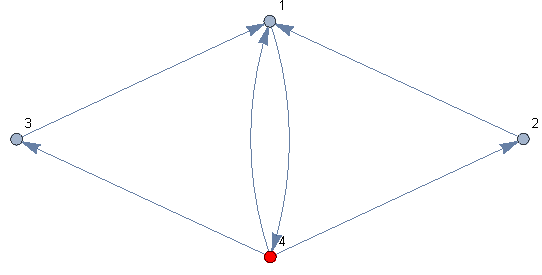
\includegraphics[width=\textwidth]{images/jackson_graph_1.pdf}
        \caption{Simple Jackson Network}
        \label{fig:jackson_graph_1}
    \end{subfigure}
    \hfill
    \begin{subfigure}[b]{0.45\textwidth}
        \centering
        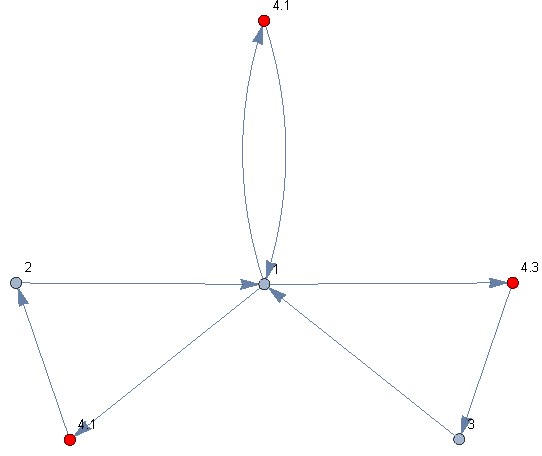
\includegraphics[width=\textwidth]{images/jackson_graph_2.pdf}
        \caption{After specializtion over vertex 4}
        \label{fig:jackson_graph_2}
    \end{subfigure}
    \hfill
       \caption{A simple Jackson traffic network model}
       \label{fig:jackson_graph}
\end{figure}

\begin{figure}
    \centering
    \begin{subfigure}[b]{0.45\textwidth}
        \centering
        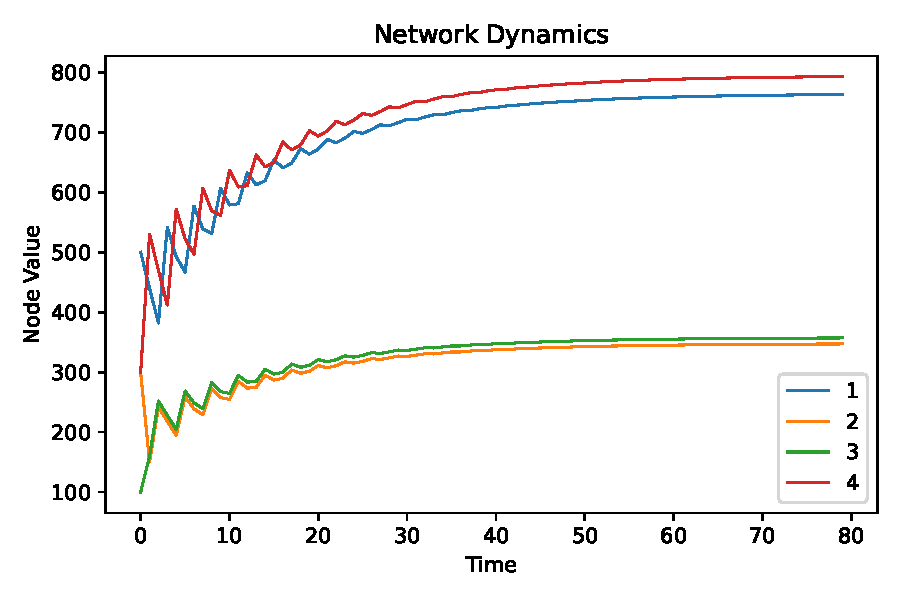
\includegraphics[width=\textwidth]{images/jackson_network_1.pdf}
        \caption{Dynamics on the original network}
        \label{fig:jackson_network_1}
    \end{subfigure}
    \hfill
    \begin{subfigure}[b]{0.45\textwidth}
        \centering
        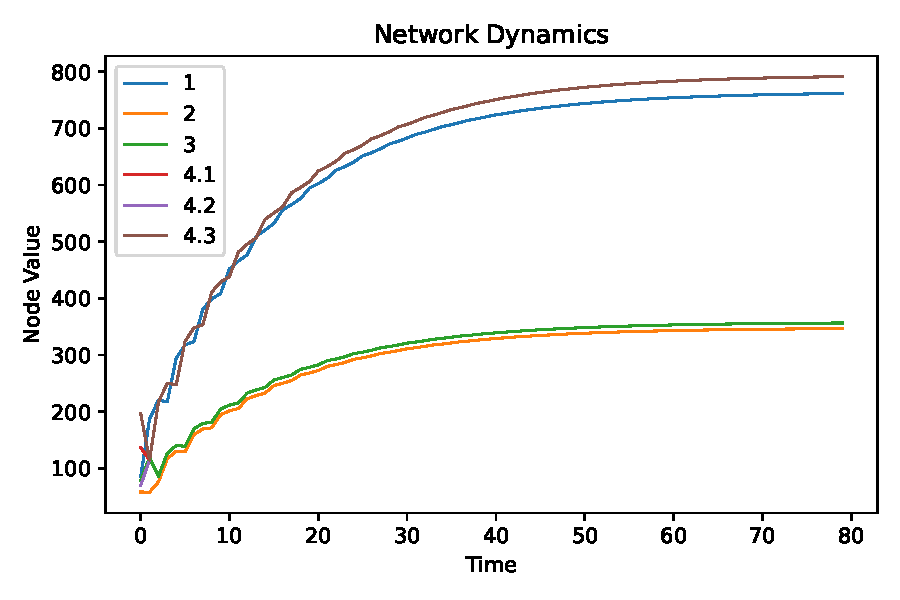
\includegraphics[width=\textwidth]{images/jackson_network_2.pdf}
        \caption{Dynamics on the specialized network}
        \label{fig:jackson_network_2}
    \end{subfigure}
    \hfill
       \caption{Dynamics on the Jackson traffic network example}
       \label{fig:jackson_network}
\end{figure}

Applying specialization to our network according to the rules outlined in this work, we can see that the network is no longer a Jackson network as the columns of $\bar{P}$ are occasionally greater than 1, so it is no longer column substochastic.

Because of this issue, we propose an addition to the specialization algorithm.
We examine one branch of the specialization process. 
We have a specialized branch $\beta = \{i, e_{i\bar{k}}, G_S, e_{\bar{\ell}j}, j \}$, upon specialization, we set $\bar{P}_{\bar{k}i} = P_{ki}P_{j\ell}/\sum_{e_{st}\in E_{S}^{{\text{out}}}}P_{st}$ and $P_{j\bar{\ell}} = P_{\ell j}$.
We will also set $\bar{\gamma}_{\bar{k}} = \gamma_{k}/|B_S(G)|$.
Applying this extended process, specializing on the same set results in the following network
\begin{align*}
    \bar{P} = 
    \begin{bmatrix} 
          0  &  0.9  &  0.9  &  0.1  &    0  &    0 \\
          0  &    0  &    0  &    0  &  0.4  &    0 \\
          0  &    0  &    0  &    0  &    0  &  0.4 \\
        0.1  &    0  &    0  &    0  &    0  &    0 \\
        0.4  &    0  &    0  &    0  &    0  &    0 \\
        0.4  &    0  &    0  &    0  &    0  &    0 
    \end{bmatrix}
    \bar{\gamma} = \begin{bmatrix} 50 \\ 30 \\ 40 \\ 10 \\ 10 \\ 10 \end{bmatrix}
\end{align*}
and we can see the resulting dynamics in Figure \ref{fig:jackson_network_fixed}.

\begin{figure}
    \centering
    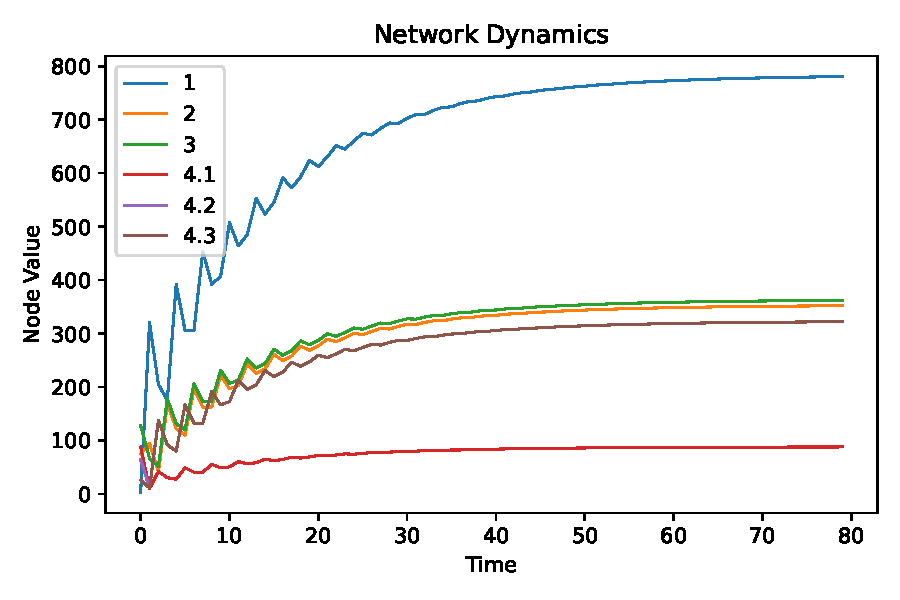
\includegraphics[width=.75\textwidth]{images/jackson_network_2_fixed.pdf}
    \caption{
        After we extend the specialization algorithm to allow network dynamics to affect it, we see what can be interpreted as significantly decreased congestion on our model traffic network.
    }
    \label{fig:jackson_network_fixed}
\end{figure}

Note that each of the column sums are less than or equal to 1, so the properties of the Jackson network are preserved.
This method further extends how we allow network dynamics to influence specialization by altering the functions in our dynamical system.
Other similar extensions may be examined, adapting the method to the type of network being considered.
In the case of Jackson networks, this product described is natural because of the properties of probabilities, another model may lead to another method natural to that model.

In real world networks there is a complex interplay between network dynamics and network growth.
The alterations and extensions to the specialization model we have explored in this chapter may allow the model to capture more real world phenomena. 
It may also empower the model with more explanatory power.
Because it links network growth to dynamics, analysis of networks after specialization may provide more insight to the dynamics of the network and make specialization more applicable to real world modeling.



\chapter{Conclusion}\label{chapt:conclusion}

In this paper we consider the interplay of the {dynamics of} and the {dynamics on} a network. We describe how the specialization model, which is used to evolve the structure of a network, leads to the formation of nontrivial equitable partitions. As the elements of these partitions form clusters that can synchronize, this structural growth has a direct impact on the {dynamics on} the network. That is, as opposed to mechanical, gravitational, or other natural forces;  specialization is a topological mechanism that induces spontaneous synchronization in dynamical networks.   

%The clusters created by specialization consist of vertices that both occupy the same relative position within their respective community and have, at least potentially, the same of dynamics. Because of this these vertices can be thought of as playing the same type of role within the network. This suggests that vertices in the same equitable partition or those vertices that synchronize in real-world networks may have the same role within their respective communities. Additionally, as each community is in fact different, the roles within them are also distinct meaning that each role in a newly specialized community is a specialized version of the original role. 

Our original motivation for considering network specialization is that it results in a number of features consistent with those observed in real-world networks. Specifically, if a network is sequentially specialized it becomes increasingly real-world like so long as the sets over which it is specialized are chosen at random \cite{8}. Although we only formally describe how a single network specialization creates or maintains equitable partitions the results in this paper can also be used to describe how an equitable partition evolves over a sequence of specializations (see Theorems \ref{thm:coarse} and \ref{thm:part_conv}).

Last, we note that the model described in this paper is not a fully integrated model of the {dynamics on} and the {dynamics of} a network. As shown, specializing a dynamical network causes changes in the dynamics on the network but these dynamics are not the cause of network specialization. Currently, it is an open question as to whether a model can be devised where the set $S$ to be specialized is chosen using the dynamics of the network and specifically whether such a model could result in both a structure and dynamic consistent with observations of real-world networks.


%%%%%%%%%%%%%%%%%%%%%%%%%%%%%%%%%%%%%%%%%%%%%%%%%%%%%%%%%%%%%%%%%%%%%%%%%%%%%%%%%%%%%%%%%%
%% \appendix changes the numbering of chapters and sections for appendices. Any chapters or 
%% sections listed here will be treated as part of the appendix
\appendix

%% Choose your bibliography style. Some options: plain, unsrt, abbrev etc.
% \bibliographystyle{unsrt}
%% the name of your bib file without the .bib extension. For example, if your file is thesis.bib, you would put \bibliography{thesis}
% \bibliography{thesis}

\begin{thebibliography}{99}
    \bibitem{11} A. B. Siddique, L. Pecora, J. D. Hart, and F. Sorrentino, Symmetry- and input-cluster synchronization in networks. \textit{Phys. Rev. E} 97, 042217, (2018).
    
    \bibitem{5} A. Ghaffarizadeh, N. S. Flann, and G. J. Podgorski, Multistable switches and their role in cellular differentiation networks. \textit{BMC Bioinformatics},PMID: 25078021 (2014).
    
    \bibitem{14} C. Coux, R. Rader, I. Bartomeus, and J. M. Tylianakis, Linking species functional roles to their network roles. \textit{Ecology letters}, Volume 19(7), (2016).
    
    \bibitem{Esp10} C. Espinosa-Soto, A. Wagner, Specialization Can Drive the Evolution of Modularity. PLoS ComputBiol, 6(3), (2010).
    
    \bibitem{Godsil01} C. Godsil and G.F. Royle, Algebraic Graph Theory. \textit{Graduate Texts in Mathematics}. Springer New York, (2001).
    
    \bibitem{6} D. A. Oyarzún, M. Chaves, M. Hoff-Hoffmeyer-Zlotnik, Multistability and oscillations in genetic control of metabolism, \textit{Journal of Theoretical Biology}, Volume 295, {139-153}, (2012).
    
    \bibitem{Povinelli95} D. J. Povinelli, and T. M. Preuss, Theory of mind: evolutionary history of a cognitive specialization. \textit{Trends in Neurosciences}, 18(9), 418-424, (1995).
    
    \bibitem{Lund21} D. Lund, J. Drapeau, B. Webb, Fourier decompositions of graphs with symmetries and equitable partitions, \textit{Linear Algebra and its Applications}, Vol. 627, {199-226}, (2021).
    
    \bibitem{Herskowitz89} I. Herskowitz, A regulatory hierarchy for cell specialization in yeast. \textit{Nature}, 342(6251), 749-757, (1989).
    
    \bibitem{3} J. Boiko, I. Pyatin, O. Eromenko, O. Barabash, Methodology for Assessing Synchronization Conditions in Telecommunication Devices, \textit{Advances in Science, Technology and Engineering Systems Journal}, vol. 5, no. 2,{320-327, (2020)}
    
    \bibitem{Fan05} J. Fan and X. Wang, On synchronization in scale-free dynamical networks. \textit{Physica A-statistical Mechanics and Its Applications}, Vol. 349, issue 3, {443-451}, (2005).
    
    \bibitem{1} J. Hasty, A. Hoffmann, and S. Golden, Systems biology of cellular rhythms: from cacophony to symphony. \textit{Current opinion in genetics and development} {20(6), 571-573, (2010).}
    
    \bibitem{13} J. Scripps, T. Pang-Ning, and A.-H. Esfahanian, Node Roles and Community Structure in Networks, \textit{Association for Computing Machinery} New York, NY, USA, (2007).
    
    \bibitem{Stelling02} J. Stelling, S. Klamt, K. Bettenbrock, S. Schuster, and E. D. Gilles, Metabolic Network Structure Determines Key Aspects of Functionality and Regulation.\textit{Nature}, {420, 190-193}, (2002).
    
    \bibitem{8} L. A. Bunimovich, D. C. Smith, and B. Z. Webb, Specialization Models of Network Growth, \textit{Journal of Complex Networks}, Volume 7, Issue 3, {375-392}, (2019).
    
    \bibitem{Bunimovich20} L. Bunimovich, D. J. Passey, D. Smith, and B. Webb, Spectral and Dynamic Consequences of Network Specialization. International Journal of Bifurcation and Chaos, 30(06), 2050091, (2020).
    
    \bibitem{2} L. Glass, Synchronization and rhythmic processes in physiology. \textit{Nature} {410, 277-284, (2001),}
    
    \bibitem{15} L. Peel, Active discovery of network roles for predicting the classes of network nodes. \textit{Journal of Complex Networks}, {3(3), 431-449}, (2015).

    \bibitem{10} L. V. Gambuzza and M. Frasca, A criterion for stability of cluster synchronization in networks with external equitable partitions. \textit{Automatica}, Volume 100, {212-218}, (2019).
    
    \bibitem{Cohen83} M. A. Cohen and S. Grossberg, Absolute stability of global pattern formation and parallel memory storage by competitive neural networks. \textit{IEEE Transactions on Systems, Man, and Cybernetics}, Vol. SMC-13, No. 5, {815-826}, (1983).

    \bibitem{12} M. A. D. Aguiar and A. P. S. Dias, Synchronization and equitable partitions in weighted networks. \textit{Chaos} 28, {073105} (2018).

    \bibitem{7} M. Newman, A.-L. Barabási, and D. J. Watts, The Structure and Dynamics of Networks, \textit{Princeton: Princeton University Press}, (2011). %{167-182}, 

    \bibitem{Newman10} M. Newman, Networks: An Introduction, \textit{Oxford University Press} {304-340, 494-568, 434-493, 108-109}, (2010).

    \bibitem{Nikolic17} N. Nikolic, F. Schreiber, A. Dal Co, D. J. Kiviet, T. Bergmiller, S. Littmann, M. Kuypers, and M. Ackermann, Cell-to-cell variation and specialization in sugar metabolism in clonal bacterial populations. \textit{PLOS Genetics}, 13(12), 1-24, (2017).
    
    \bibitem{Prulzj07} N. Przulj, Biological Network Comparison using Graphlet Degree Distribution. \textit{Bioinformatics}, Vol. 23, Issue 2, {177-183} (2007).

    \bibitem{Sporns13} O. Sporns, Network attributes for segregation and integration in the human brain. \textit{Curr. Opin. Neurobiol.} PMID: 23294553, {162-171}, (2013).

    \bibitem{Salz01} R. J. Salz and D. K. Loomis, and K. L. Finn, Development and Validation of a Specialization Index and Testing of Specialization Theory. \textit{Human Dimensions of Wildlife}, 6(4), 239-258, (2001).

    \bibitem{9} R. V. Solé V and S. Valverde, Spontaneous emergence of modularity in cellular networks. \textit{J. R. Soc. Interface} 5129-133, {129-133}, (2008).

    \bibitem{4} S. Bregni, Synchronization of Digital Telecommunications Networks. \textit{John Wiley and Sons}, Ltd, {171-179}, (2002).

    \bibitem{Wang02} X. F. Wang and G. Chen, Synchronization in scale-free dynamical networks: robustness and fragility. \textit{IEEE Transactions on Circuits and Systems I: Fundamental Theory and Applications}, Vol. 49, No. 1, {54-62}, (2002).
\end{thebibliography}

%% If you want to include an index, this prints the index at this location. You must 
%% have \makeindex uncommented in the preamble
% \printindex

\end{document}
